%%%%%%%%%%%%%%%%%%%%%%%%%%%%%%%%%%%%%%%%%%%%%%%%%%%%%%%%%%%%%%%
%% OXFORD THESIS TEMPLATE

% Use this template to produce a standard thesis that meets the Oxford University requirements for DPhil submission
%
% Originally by Keith A. Gillow (gillow@maths.ox.ac.uk), 1997
% Modified by Sam Evans (sam@samuelevansresearch.org), 2007
% Modified by John McManigle (john@oxfordechoes.com), 2015
% Modified by Ulrik Lyngs (ulrik.lyngs@cs.ox.ac.uk), 2018-, for use with R Markdown
%
% Ulrik Lyngs, 25 Nov 2018: Following John McManigle, broad permissions are granted to use, modify, and distribute this software
% as specified in the MIT License included in this distribution's LICENSE file.
%
% John commented this file extensively, so read through to see how to use the various options.  Remember that in LaTeX,
% any line starting with a % is NOT executed.  Several places below, you have a choice of which line to use
% out of multiple options (eg draft vs final, for PDF vs for binding, etc.)  When you pick one, add a % to the beginning of
% the lines you don't want.


%%%%% PAGE LAYOUT
% The most common choices should be below.  You can also do other things, like replacing "a4paper" with "letterpaper", etc.

% This one formats for two-sided binding (ie left and right pages have mirror margins; blank pages inserted where needed):
%\documentclass[a4paper,twoside]{templates/ociamthesis}
% This one formats for one-sided binding (ie left margin > right margin; no extra blank pages):
%\documentclass[a4paper]{ociamthesis}
% This one formats for PDF output (ie equal margins, no extra blank pages):
%\documentclass[a4paper,nobind]{templates/ociamthesis}

% As you can see from the uncommented line below, oxforddown template uses the a4paper size, 
% and passes in the binding option from the YAML header in index.Rmd:
\documentclass[a4paper, nobind]{templates/ociamthesis}


%%%%% ADDING LATEX PACKAGES
% add hyperref package with options from YAML %
\usepackage[pdfpagelabels]{hyperref}
% change the default coloring of links to something sensible
\usepackage{xcolor}
\usepackage[hangul]{kotex}


\definecolor{mylinkcolor}{RGB}{0,0,139}
\definecolor{myurlcolor}{RGB}{0,0,139}
\definecolor{mycitecolor}{RGB}{0,33,71}

\hypersetup{
  hidelinks,
  colorlinks,
  linktocpage=true,
  linkcolor=mylinkcolor,
  urlcolor=myurlcolor,
  citecolor=mycitecolor
}



% add float package to allow manual control of figure positioning %
\usepackage{float}

% enable strikethrough
\usepackage[normalem]{ulem}

% use soul package for correction highlighting
\usepackage{color, soul}
\definecolor{correctioncolor}{HTML}{CCCCFF}
\sethlcolor{correctioncolor}
\newcommand{\ctext}[3][RGB]{%
  \begingroup
  \definecolor{hlcolor}{#1}{#2}\sethlcolor{hlcolor}%
  \hl{#3}%
  \endgroup
}
\soulregister\ref7
\soulregister\cite7
\soulregister\autocite7
\soulregister\textcite7
\soulregister\pageref7

%%%%% FIXING / ADDING THINGS THAT'S SPECIAL TO R MARKDOWN'S USE OF LATEX TEMPLATES
% pandoc puts lists in 'tightlist' command when no space between bullet points in Rmd file,
% so we add this command to the template
\providecommand{\tightlist}{%
  \setlength{\itemsep}{0pt}\setlength{\parskip}{0pt}}
 
% UL 1 Dec 2018, fix to include code in shaded environments

% User-included things with header_includes or in_header will appear here
% kableExtra packages will appear here if you use library(kableExtra)
\usepackage{booktabs}
\usepackage{longtable}
\usepackage{array}
\usepackage{multirow}
\usepackage{wrapfig}
\usepackage{float}
\usepackage{colortbl}
\usepackage{pdflscape}
\usepackage{tabu}
\usepackage{threeparttable}
\usepackage{threeparttablex}
\usepackage[normalem]{ulem}
\usepackage{makecell}
\usepackage{xcolor}


%UL set section header spacing
\usepackage{titlesec}
% 
\titlespacing\subsubsection{0pt}{24pt plus 4pt minus 2pt}{0pt plus 2pt minus 2pt}


%UL set whitespace around verbatim environments
\usepackage{etoolbox}
\makeatletter
\preto{\@verbatim}{\topsep=0pt \partopsep=0pt }
\makeatother



%%%%%%% PAGE HEADERS AND FOOTERS %%%%%%%%%
\usepackage{fancyhdr}
\setlength{\headheight}{15pt}
\fancyhf{} % clear the header and footers
\pagestyle{fancy}
\renewcommand{\chaptermark}[1]{\markboth{\thechapter. #1}{\thechapter. #1}}
\renewcommand{\sectionmark}[1]{\markright{\thesection. #1}} 
\renewcommand{\headrulewidth}{0pt}

\fancyhead[LO]{\emph{\leftmark}} 
\fancyhead[RE]{\emph{\rightmark}} 

% UL page number position 
\fancyfoot[R]{\emph{\thepage}} %regular pages
\fancypagestyle{plain}{\fancyhf{}\fancyfoot[R]{\emph{\thepage}}} %chapter pages

% JEM fix header on cleared pages for openright
\def\cleardoublepage{\clearpage\if@twoside \ifodd\c@page\else
   \hbox{}
   \fancyfoot[R]{}
   \newpage
   \if@twocolumn\hbox{}\newpage
   \fi
   \fancyhead[LO]{\emph{\leftmark}} 
   \fancyhead[RE]{\emph{\rightmark}} 
   \fi\fi}


%%%%% SELECT YOUR DRAFT OPTIONS
% This adds a "DRAFT" footer to every normal page.  (The first page of each chapter is not a "normal" page.)

% IP feb 2021: option to include line numbers in PDF

% This highlights (in blue) corrections marked with (for words) \mccorrect{blah} or (for whole
% paragraphs) \begin{mccorrection} . . . \end{mccorrection}.  This can be useful for sending a PDF of
% your corrected thesis to your examiners for review.  Turn it off, and the blue disappears.
\correctionstrue


%%%%% BIBLIOGRAPHY SETUP
% Note that your bibliography will require some tweaking depending on your department, preferred format, etc.
% If you've not used LaTeX before, I recommend reading a little about biblatex/biber and getting started with it.
% If you're already a LaTeX pro and are used to natbib or something, modify as necessary.
% Either way, you'll have to choose and configure an appropriate bibliography format...


\usepackage[style=authoryear, sorting=nyt, backend=biber, maxcitenames=2, useprefix, doi=true, isbn=false, uniquename=false]{biblatex}
\newcommand*{\bibtitle}{Works Cited}

\addbibresource{bibliography/references.bib}
\addbibresource{bibliography/additional-references.bib}


% This makes the bibliography left-aligned (not 'justified') and slightly smaller font.
\renewcommand*{\bibfont}{\raggedright\small}


% Uncomment this if you want equation numbers per section (2.3.12), instead of per chapter (2.18):
%\numberwithin{equation}{subsection}


%%%%% THESIS / TITLE PAGE INFORMATION
% Everybody needs to complete the following:
\title{Uplift Resistance of Anchor Plate Using Extended Mohr-Coulomb Model}
\author{Kyeong Sun Kim}
\college{Civil and Environmental Engineering}

% Master's candidates who require the alternate title page (with candidate number and word count)
% must also un-comment and complete the following three lines:

% Uncomment the following line if your degree also includes exams (eg most masters):
%\renewcommand{\submittedtext}{Submitted in partial completion of the}
% Your full degree name.  (But remember that DPhils aren't "in" anything.  They're just DPhils.)
\degree{}
% Term and year of submission, or date if your board requires (eg most masters)
\degreedate{November, 2021}


%%%%% YOUR OWN PERSONAL MACROS
% This is a good place to dump your own LaTeX macros as they come up.

% To make text superscripts shortcuts
	\renewcommand{\th}{\textsuperscript{th}} % ex: I won 4\th place
	\newcommand{\nd}{\textsuperscript{nd}}
	\renewcommand{\st}{\textsuperscript{st}}
	\newcommand{\rd}{\textsuperscript{rd}}

%%%%% THE ACTUAL DOCUMENT STARTS HERE
\begin{document}

%%%%% CHOOSE YOUR LINE SPACING HERE
% This is the official option.  Use it for your submission copy and library copy:
\setlength{\textbaselineskip}{22pt plus2pt}
% This is closer spacing (about 1.5-spaced) that you might prefer for your personal copies:
%\setlength{\textbaselineskip}{18pt plus2pt minus1pt}

% You can set the spacing here for the roman-numbered pages (acknowledgements, table of contents, etc.)
\setlength{\frontmatterbaselineskip}{17pt plus1pt minus1pt}

% UL: You can set the line and paragraph spacing here for the separate abstract page to be handed in to Examination schools
\setlength{\abstractseparatelineskip}{13pt plus1pt minus1pt}
\setlength{\abstractseparateparskip}{0pt plus 1pt}

% UL: You can set the general paragraph spacing here - I've set it to 2pt (was 0) so
% it's less claustrophobic
\setlength{\parskip}{2pt plus 1pt}

%
% Oxford University logo on title page
%
\def\crest{{\includegraphics[width=5cm]{templates/snupdf.pdf}}}
\renewcommand{\university}{Seoul National University}
\renewcommand{\submittedtext}{}


% Leave this line alone; it gets things started for the real document.
\setlength{\baselineskip}{\textbaselineskip}


%%%%% CHOOSE YOUR SECTION NUMBERING DEPTH HERE
% You have two choices.  First, how far down are sections numbered?  (Below that, they're named but
% don't get numbers.)  Second, what level of section appears in the table of contents?  These don't have
% to match: you can have numbered sections that don't show up in the ToC, or unnumbered sections that
% do.  Throughout, 0 = chapter; 1 = section; 2 = subsection; 3 = subsubsection, 4 = paragraph...

% The level that gets a number:
\setcounter{secnumdepth}{2}
% The level that shows up in the ToC:
\setcounter{tocdepth}{2}


%%%%% ABSTRACT SEPARATE
% This is used to create the separate, one-page abstract that you are required to hand into the Exam
% Schools.  You can comment it out to generate a PDF for printing or whatnot.

% JEM: Pages are roman numbered from here, though page numbers are invisible until ToC.  This is in
% keeping with most typesetting conventions.
\begin{romanpages}

% Title page is created here
\maketitle

%%%%% DEDICATION -- If you'd like one, un-comment the following.

%%%%% ACKNOWLEDGEMENTS -- Nothing to do here except comment out if you don't want it.


%%%%% ABSTRACT -- Nothing to do here except comment out if you don't want it.
%\begin{abstract}
%	
%\end{abstract}

%%%%% MINI TABLES
% This lays the groundwork for per-chapter, mini tables of contents.  Comment the following line
% (and remove \minitoc from the chapter files) if you don't want this.  Un-comment either of the
% next two lines if you want a per-chapter list of figures or tables.
  \dominitoc % include a mini table of contents

% This aligns the bottom of the text of each page.  It generally makes things look better.
\flushbottom

% This is where the whole-document ToC appears:
\tableofcontents


% Uncomment to generate a list of tables:
%%%%% LIST OF ABBREVIATIONS
% This example includes a list of abbreviations.  Look at text/abbreviations.tex to see how that file is
% formatted.  The template can handle any kind of list though, so this might be a good place for a
% glossary, etc.

% The Roman pages, like the Roman Empire, must come to its inevitable close.
\end{romanpages}

%%%%% CHAPTERS
% Add or remove any chapters you'd like here, by file name (excluding '.tex'):
\flushbottom

% all your chapters and appendices will appear here
\begin{figure}[H]
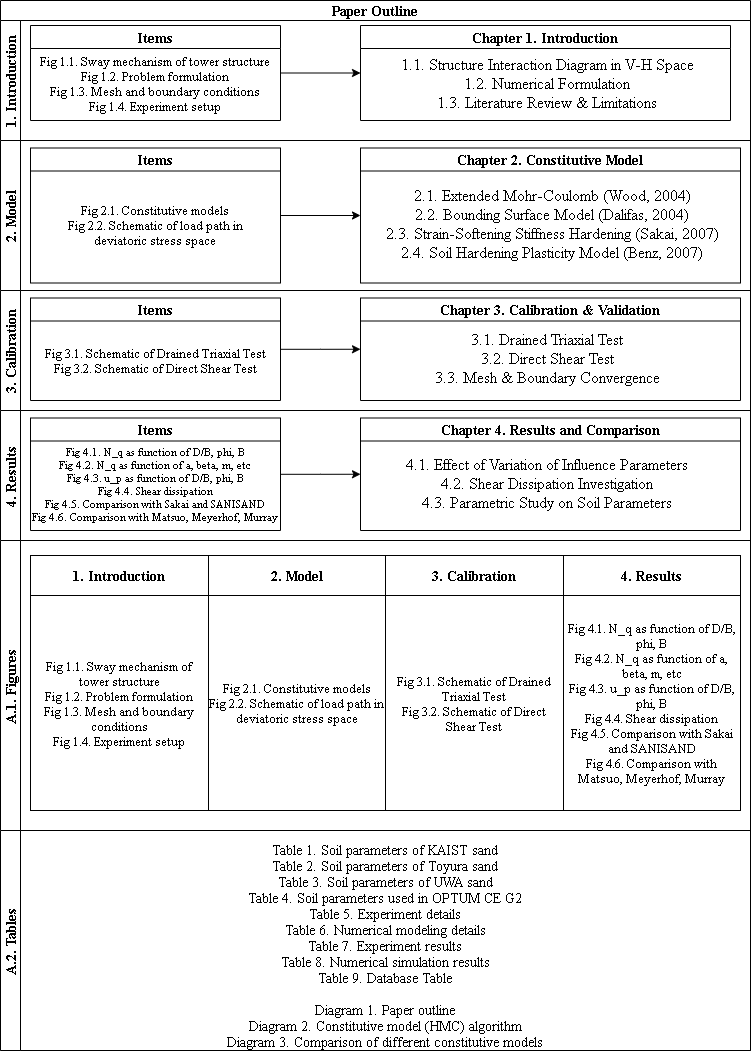
\includegraphics[width=1\linewidth]{myfigureeeeee/paper outline} \caption{Paper Outline}\label{fig:unnamed-chunk-1}
\end{figure}

\hypertarget{constitutive-model}{%
\chapter{Constitutive Model}\label{constitutive-model}}

\chaptermark{Constitutive models}
\minitoc

\newpage

\noindent Here is a brief description of the constitutive models:\\
1. Strain---Softening Stiffness---Hardening Model by Sakai and Tanaka, 1993\\
2. Typical Mohr-Coulomb with Non-associated Flow\\
3. Extended Mohr-Coulomb Model by David Muir Wood, 2004

\hypertarget{strainsoftening-stiffnesshardening-model}{%
\section{Strain---Softening Stiffness---Hardening Model}\label{strainsoftening-stiffnesshardening-model}}

It is assumed that the yield function \(F\) is defined by the stress \(\vec{\sigma}\) and the soil parameter \(\chi\) (Tanaka and Sakai, 1993):\\
\(F(\vec{\sigma},\alpha(\chi))=0\)

In order to avoid numerical instability due to singularity of the non-associated Mohr-Coulomb model, a constitutive model based on the yield function of M-C type and the plastic potential function of Draker-Prager type is employed.

For predicting deformations in a post-peak regime, the elastic- strain-softening plastic model is developed. The yield function is given by the following expression.

\hypertarget{yield-function}{%
\subsection{Yield function}\label{yield-function}}

\[
  F(\vec{\sigma},\alpha(\chi)) = 3\alpha(\chi)p'+\frac{\sqrt{J_2}}{g(\theta)}-c(\chi) = 0
\]

\hypertarget{plastic-potential-function}{%
\subsection{Plastic potential function}\label{plastic-potential-function}}

\[
  G(\vec{\sigma},\alpha'(\chi)) = 3\alpha^{'}(\chi)p'+\sqrt{J_2}-c(\chi) = 0
\]

\[
  \chi = \int \delta\varepsilon^{p}
\]

\[
  (\delta\varepsilon^{p})^2 = 2[(\delta\epsilon_x^{p})^2+(\delta\epsilon_y^{p})^2+(\delta\epsilon_z^{p})^2+]+(\delta\gamma^{p})^2
\]
, where\\
\(p^{'}\) is mean stress,\\
\(J_2\) is second invariant of deviatoric stress,\\
\(\chi\) is soil hardening parameter,\\
\(c(\chi)\) is apparent cohesion function,\\
\(\delta \varepsilon_{x,y,z}^{p} , \delta \gamma^{p}\) is incremental deviatoric plastic strains.

In case of the Mohr-Coulomb model, \(g(\theta)\) is given by:

\[
  g(\theta) = \frac{3-sin\phi}{2\sqrt{3}cos\theta -2sin\theta sin\phi}
\]
, where\\
\(\theta\) is Lode angle; if triaxial compression, \(=-30 ^{\circ}\)\\
\(\phi\) is mobilized internal friction angle.

\hypertarget{hardening-function}{%
\subsection{Hardening function}\label{hardening-function}}

The simple strain-softening functions are specified and expressed as a function of material constants. (Tanaka and Sakai, 1993)

\[
\alpha(\chi) = {(\frac{2\sqrt{a\chi }}{\chi +a})}^m \alpha_p\; \\ (hardening \; regime;\; \chi \leq a) 
\]

\[
\alpha(\chi) = \alpha_r + (\alpha_p - \alpha_r) exp\{-(\frac{\chi-a}{b})\}\; \\ (softening \; regime;\; \chi > a) 
\]
, where\\
\(a, b, m\) are soil parameters.

Similar expressions are used by de Borst (1986).

\[
\alpha_p = \frac{2 sin \phi_p}{\sqrt{3}(3-sin\phi_p)}
\]

\[
\alpha_r = \frac{2 sin \phi_r}{\sqrt{3}(3-sin\phi_r)}
\]
, where\\
\(\phi_{p,r}\) are peak and residual friction angle, respectively.

\hypertarget{nonassociated-flow-rule-na}{%
\section{Nonassociated Flow Rule (NA)}\label{nonassociated-flow-rule-na}}

Since there may be a range of possible solutions, each associated with a different pattern of localization and all of which are entirely valid, it can be expected that any numerical solution will be very sensitive to both physical imperfections as well as round-off errors and the exact sequence in which the procedures defining the solution scheme are carried out. In the end, the result is a load-displacement response that tends to be rather oscillatory.

\begin{figure}[H]
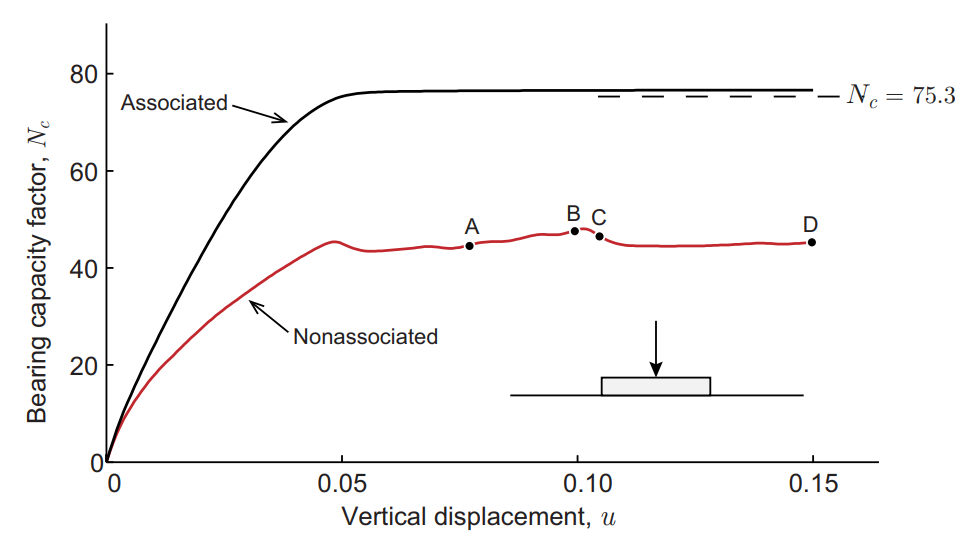
\includegraphics[width=1\linewidth]{myfigureeeeee/Load-displacement response for strip footing on a weightless soil} \caption{Load-displacement response for strip footing on a weightless soil (After  Krabbenhoft et al., 2012)}\label{fig:unnamed-chunk-2}
\end{figure}

The basic idea behind the formulation derives from the structure of the internal dissipation associated with constitutive models. Let us assume a yield function of the type:

\[
F = Mp+q-c
\]
, where\\
\(p\) and \(q\) are mean and deviatoric stress, \(M\) is a friction coeffcieint, and \(c\) is cohesion.

The plastic potential function is given by:\\
\[
G = Np +q
\]
, where \(N \leq M\) is a dilation coefficient.

In \(p-q\) triaxial space, the plastic strain rates are given by:

\[
\delta \varepsilon_v^{p} = \delta \lambda \frac{\partial G}{\partial p} = \delta \lambda N \\
\delta \varepsilon_s^{p} = \delta \lambda \frac{\partial G}{\partial p} = \delta \lambda
\]
, where
\(\delta\) denotes time increment, \(\varepsilon_v^{p}\) and \(\varepsilon_s^{p}\) are volumetic and deviatoric plastic strains conjugate to \(p\) and \(q\), respectively.

The dissipation \(D\) is given by:

\(\begin{aligned} D &= p \varepsilon_v^{p} + q \varepsilon_s^{p} \\  &= (Nq+q) \delta \lambda \\  &= [c-(M-N)p]\delta \lambda \\  &= [c - (M-N)p]\varepsilon_s^{p} \end{aligned}\)

The above-mentioned parameters are all related with the confining pressure, which can be easily illustraed with the figure below:

\begin{figure}[H]
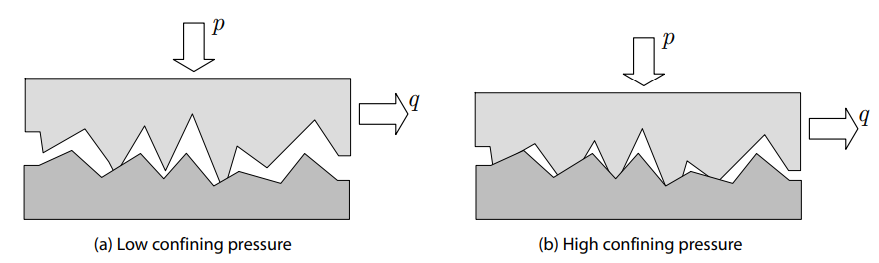
\includegraphics[width=1\linewidth]{myfigureeeeee/confiningpressure} \caption{Microscopic origins of friction as plastic shearing of asperities. A higher confining pressure implies a higher degree of interlocking of the asperities and thereby a higher apparent shear strength (After  Krabbenhoft et al., 2012)}\label{fig:unnamed-chunk-3}
\end{figure}

\hypertarget{extended-mohrcoulomb-model-emc}{%
\section{Extended Mohr---Coulomb Model (EMC)}\label{extended-mohrcoulomb-model-emc}}

The elastic-perfectly plastic Mohr-Coulomb model is widely used for geotechnical analysis. It provides very crude match to actual shearing behavior of soils. A natural extension is to create a hardening version of the M-C model in which the size of the yield surface varies in some nonlinear way with the development of plastic strain. In the model to be described as hardening will be linked only with distortional strain. It is useful for modelling sands , where it is rearrangement of the rather particles that dominates the response and irrecoverable volumetric changes are essentially linked by this rearrangement of particles (Wood, 2004).

\begin{figure}[H]
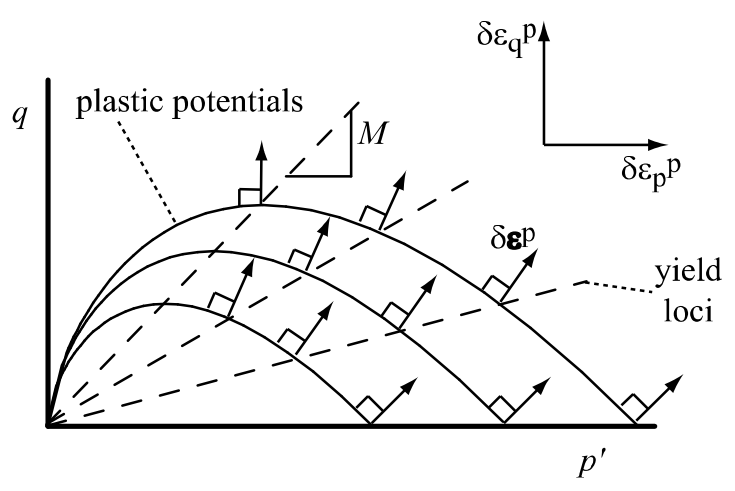
\includegraphics[width=1\linewidth]{myfigureeeeee/Plastic potential curves (solid lines) and yield loci (dashed lines) in elastic-hardening plastic Mohr-Coulomb model} \caption{Plastic potential curves (solid lines) and yield loci (dashed lines) in elastic-hardening plastic Mohr-Coulomb modele}\label{fig:unnamed-chunk-4}
\end{figure}

Following Taylor's (1948) proposal of a link between dilatancy and mobilized friction in a shear box test, stress---dilatancy equation expressed in terms of total strain increments is obtained.

\begin{figure}[H]
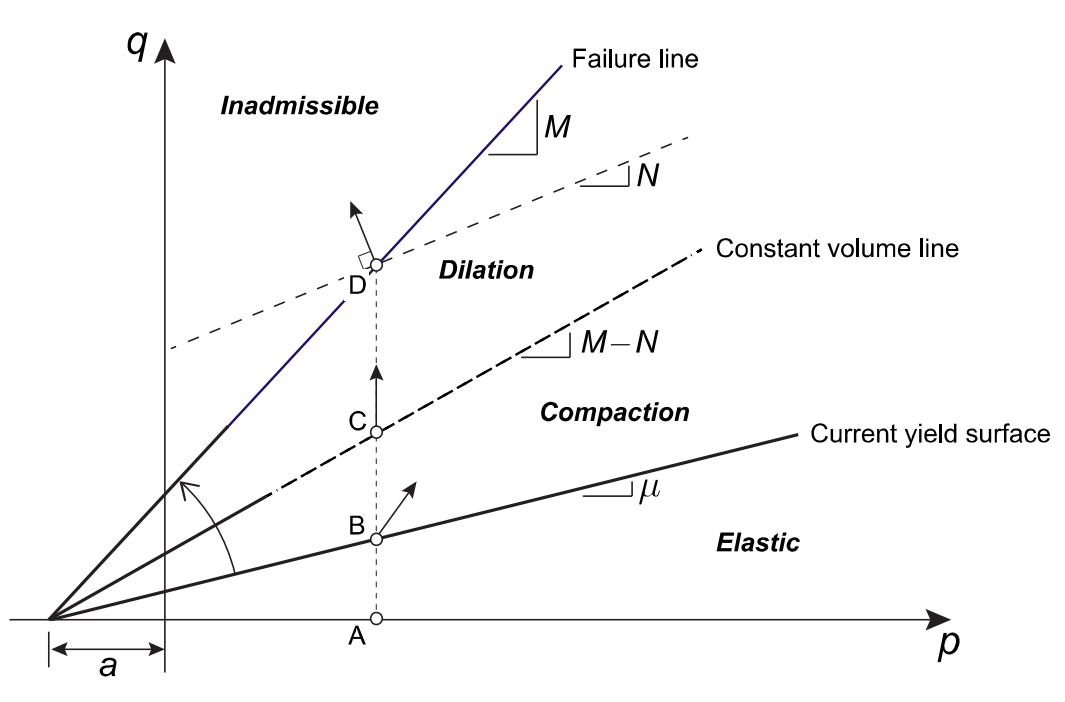
\includegraphics[width=1\linewidth]{myfigureeeeee/Hardening, compaction and dilation in the HMC model} \caption{Hardening, compaction and dilation in the HMC model}\label{fig:unnamed-chunk-5}
\end{figure}

\hypertarget{comparison-between-associated-and-non-associated-flow-rule-in-plastic-model}{%
\subsection{Comparison between associated and non-associated flow rule in plastic model}\label{comparison-between-associated-and-non-associated-flow-rule-in-plastic-model}}

In the elastic-perfectly-plastic Mohr-Coulomb model, it is commonly assumed that the plastic potential takes the same form as the yield surface, but with the slope defined by a dilation angle \(\psi\) rather than a friction angle. If this assumption is adopted, then the dirction of the plastic strain increment \(\delta \varepsilon^{p}\) would be normal to a set of parallel lines by the dilation angle. If normality rule were assumed, radical difference between the slope of yield criterion line and the plastic potental contour is observed (J.P. Doherty and D. Muir Wood, 2013).

\begin{figure}[H]
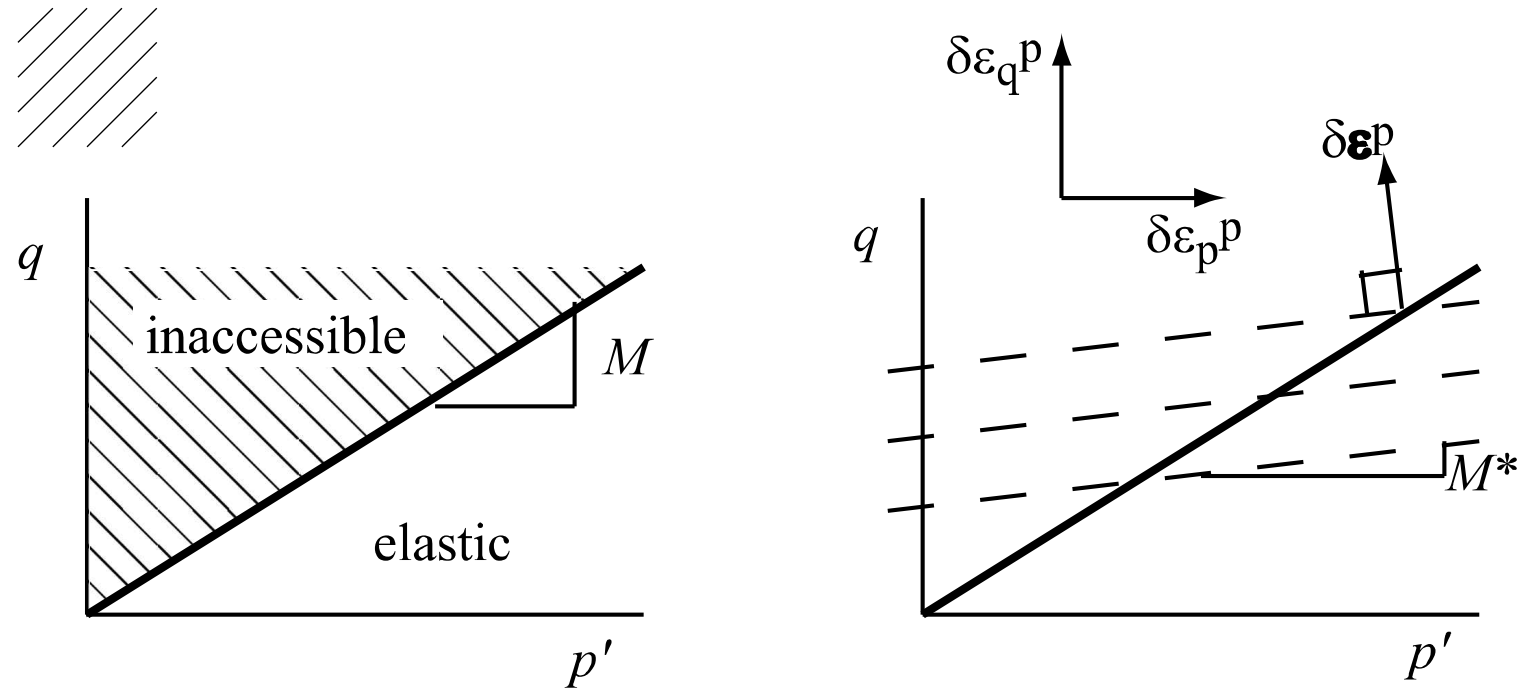
\includegraphics[width=1\linewidth]{myfigureeeeee/Elastic-perfectly plastic Mohr-Coulomb model (a) yield and failure locus, (b) plastic potentials} \caption{Elastic-perfectly plastic Mohr-Coulomb model (a) yield and failure locus, (b) plastic potentials}\label{fig:unnamed-chunk-6}
\end{figure}

\begin{figure}[H]
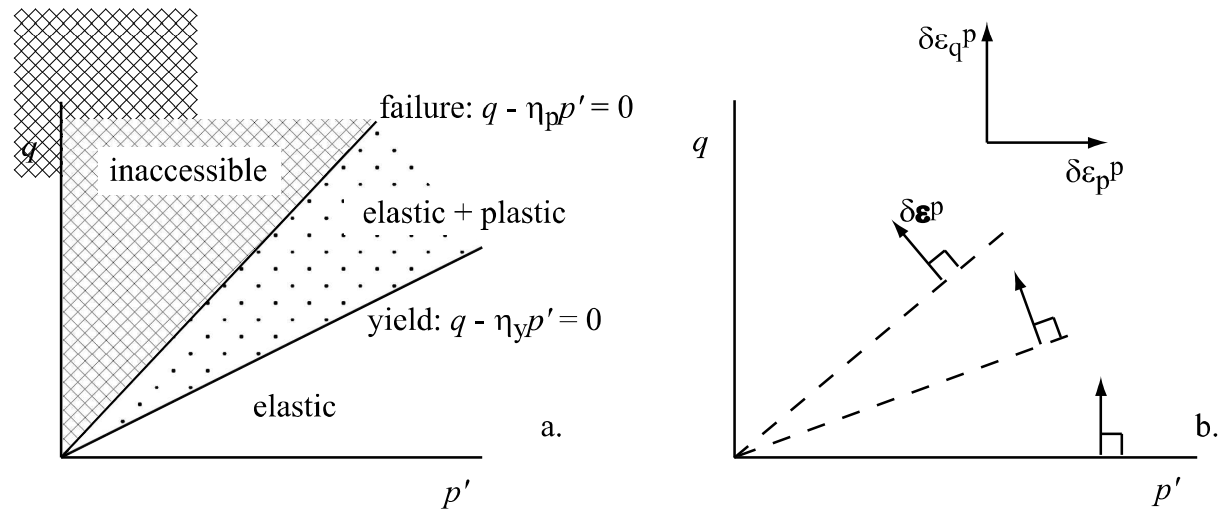
\includegraphics[width=1\linewidth]{myfigureeeeee/Elastic-hardening plastic Mohr-Coulomb model (a) yield locus and failure locus separating elastic plastic and inaccessible regions of stress plane (b) normality of pla} \caption{Elastic-hardening plastic Mohr-Coulomb model (a) yield locus and failure locus separating elastic plastic and inaccessible regions of stress plane (b) normality applied at the plastic region}\label{fig:unnamed-chunk-7}
\end{figure}

\hypertarget{yield-function-1}{%
\subsection{Yield function}\label{yield-function-1}}

\[
F(\vec{\sigma}, \chi) = F(p',q,\chi)=q - \eta_y p'=0
\]

\hypertarget{plastic-potential-function-1}{%
\subsection{Plastic potential function}\label{plastic-potential-function-1}}

\[
G(\vec{\sigma}) = q-(M -M') p' ln(\frac{p_r'}{p'})=0
\]
, where
\(\eta_{y,p}\) is stress ratio at yield and peak, respectively,\\
\(p_r'\) is chosen s.t. plastic potential gradient passes through current stress, i.e.,\\
\(p_r' = p' exp \{ \frac{\eta_y}{M-M'} \}\)\\
\(M\) is material parameter at perfect plasticity when hardening terminates.\\
\(M = \frac{6 sin \phi}{3 - sin\phi}\)\\
\(M'\) is dilation at constant volume line:\\
\(M' = \frac{6 sin \psi}{3 - sin\psi}\)\\
\(M' = M - k \psi = M-k(v-\Gamma+\lambda lnp')\)\\
\(k\) is soil constant linking state variable and strength.\\
Critical State description is as follows:\\
\(M' = M - k [(v_0 - \Gamma + \lambda ln p_0' + (\lambda ln \frac{p'}{p_0'}-v_0 \varepsilon_p^e)-v_0\varepsilon_p^p)]\).

\hypertarget{flow-rule}{%
\subsection{Flow rule}\label{flow-rule}}

\[
\frac{\delta \varepsilon_{p}^{p}}{\delta \varepsilon_{q}^{p}} = M -M'- \eta_y
\]

\hypertarget{hardening}{%
\subsection{Hardening}\label{hardening}}

\[
\delta \eta_y = \frac{1-\frac{\eta_y}{M}}{\beta} \delta \varepsilon_q^p
\]
, where\\
\(\beta\) is a model parameter scaling plastic strain,\\
\(\beta = \frac{3}{2}p' \frac{9-M}{9-(M-M')M ln2 - 3M'} \frac{1-E_{50}/E_{ur}}{E_{50}}\) for Taylor's \(\sigma-\psi\) relation.

The incremental of the stress ratio is defined as:

\(\delta \eta_y = \frac{3 sin \delta \phi}{\sqrt{3}cos\theta+sin\theta sin\delta\phi}\)

\hypertarget{soil-parameters}{%
\subsection{Soil Parameters}\label{soil-parameters}}

\hypertarget{elastic-moduli}{%
\subsubsection{Elastic Moduli}\label{elastic-moduli}}

The elastic moduli are estimated from the modified equation proposed by Hardin and Black (1968) in the case of sand:

\[
G = G_0 \frac{(2.17-e)^2}{1+e}\sqrt{p'} \\
K = \frac{1+\nu}{3(1-2 \nu)}G
\]
, where\\
\(\nu\) is Poisson's ratio,\\
\(e\) is void ratio,\\
\(G_0\) is initial shear modulus.

\hypertarget{peak-friction-angle}{%
\subsubsection{Peak friction angle}\label{peak-friction-angle}}

The peak friction angle of \(\phi_p\) is estimated from the empirical relations proposed by Bolton (1987):

\[
I_r = D_r[5-ln(\frac{p'}{150})]-1, \; (p' \geq 150 kN/m^2) \\
I_r = 5D_r -1 , \; (p' < 150 kN/m^2) \\ 
\phi_p = 3I_r + \phi_r
\]

\hypertarget{dilatency-angle}{%
\subsubsection{Dilatency angle}\label{dilatency-angle}}

The dilatency angle of \(\psi\) is estimated from modified Rowe's stress--dilatency relationship:

\[
sin\psi = \frac{sin\phi-sin\phi_r'}{1-sin\phi sin\phi_r'} \\
\phi_r' = \phi_r[1-\beta exp\{-(\frac{\chi}{\epsilon_d})^2\}]
\]
, where\\
\(\beta\) and \(\epsilon_d\) are stress---dilatency material parameters.\\
\(E_{50}\) is a secant modulus defined as:\\
\(E_{50} = \frac{\frac{1}{2}q_{u}}{\varepsilon_{a,50}}\)\\
\(E_{ur}\) is unloading/reloading stiffness.

\hypertarget{calibration}{%
\chapter{Calibration and Validation}\label{calibration}}

\chaptermark{Calibration}

\minitoc 
\noindent For the validity of the finite element tests performed, the triaxial elemental test is siumlated with the box of union length. The set up is as follows:

\hypertarget{drained-triaxial-test}{%
\section{Drained Triaxial Test}\label{drained-triaxial-test}}

\begin{figure}[H]
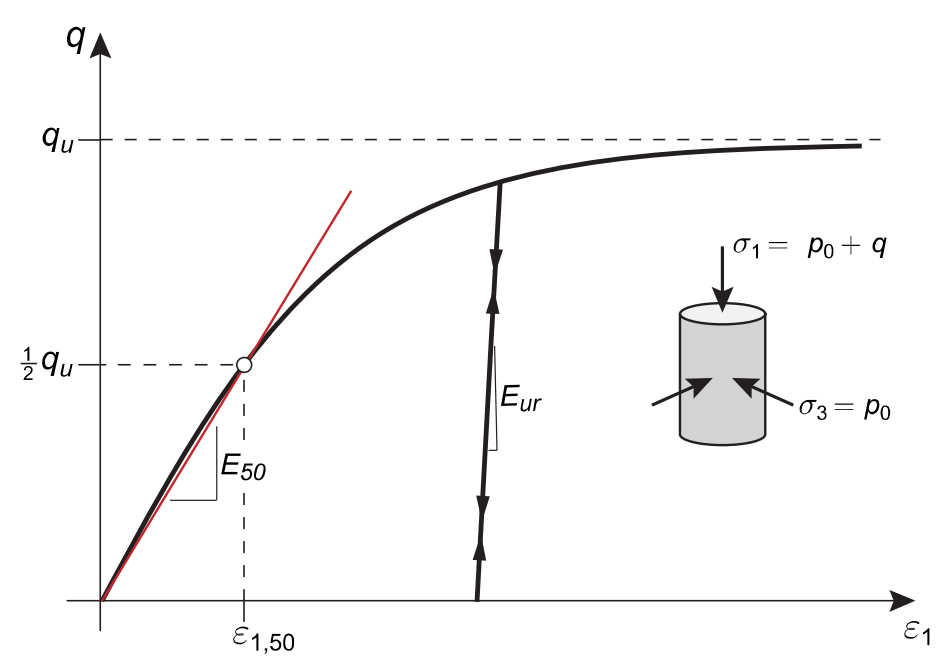
\includegraphics[width=1\linewidth]{myfigureeeeee/triaxial test} \caption{Typical triaxial test (After Krabbenhoft, 2013)}\label{fig:unnamed-chunk-8}
\end{figure}

\begin{figure}[H]
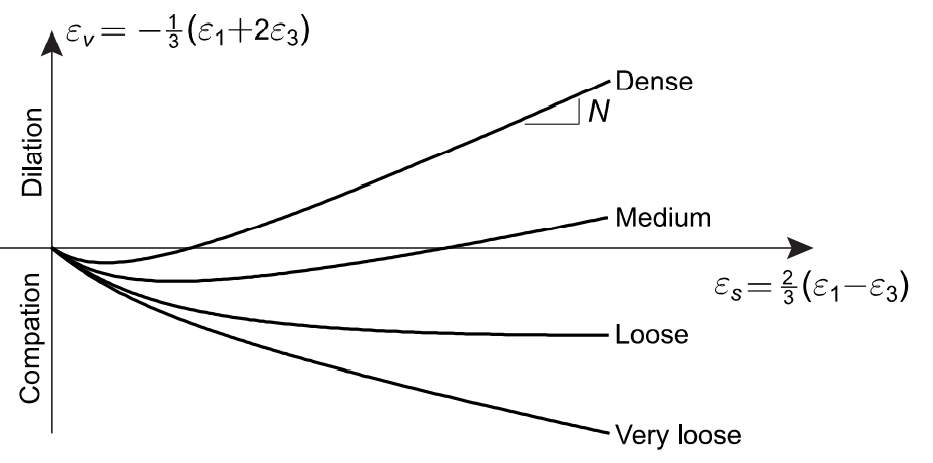
\includegraphics[width=1\linewidth]{myfigureeeeee/typical shear-volumetric strain behavior in triaxial compression} \caption{Typical shear-volumetric strain behavior in triaxial compression (After Krabbenhoft, 2013)}\label{fig:unnamed-chunk-9}
\end{figure}

Two tests --- Triaxial compression and extension (TC/TE) --- are simulated using Multiplier Elasto---plastic analysis under axisymmetric conditions as indicated in the Figure below.
The fixed loads here represent the initial axial and radial stresses while the axial Multiplier load is increased in the course of the analysis to reach the ultimate limit state.

\begin{figure}[H]
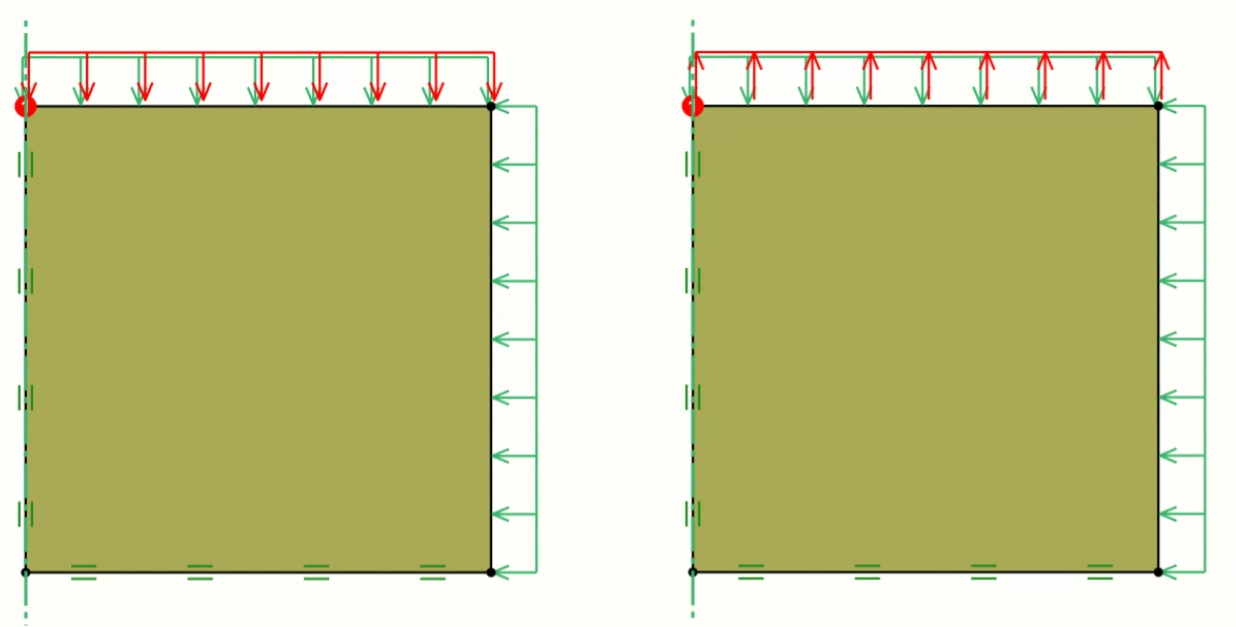
\includegraphics[width=1\linewidth]{myfigureeeeee/setup for TC and TE} \caption{Setup for elemental triaxial compression and extension}\label{fig:unnamed-chunk-10}
\end{figure}

By a process of trial and error, the fits shown in Figure are obtained. For this data set , where no information about the behavior in simple shear is available the value is well within range that can be accommodated by the isotropic strength option, there is little reason to assume any anisotropy.
We note that the compression secant modulus in compression is only half of the extension secant modulus. This is somewhat unusual, but in this case nevertheless what fits the data best.

\hypertarget{result-of-elemental-triaxial-test-at-100-kpa}{%
\subsubsection{Result of Elemental Triaxial Test at 100 kPa}\label{result-of-elemental-triaxial-test-at-100-kpa}}

Triaxial test at radial stress of 100 kPa is simulated using one by one block of the finite elmeent formulation with the EMC model.

\begin{figure}[H]
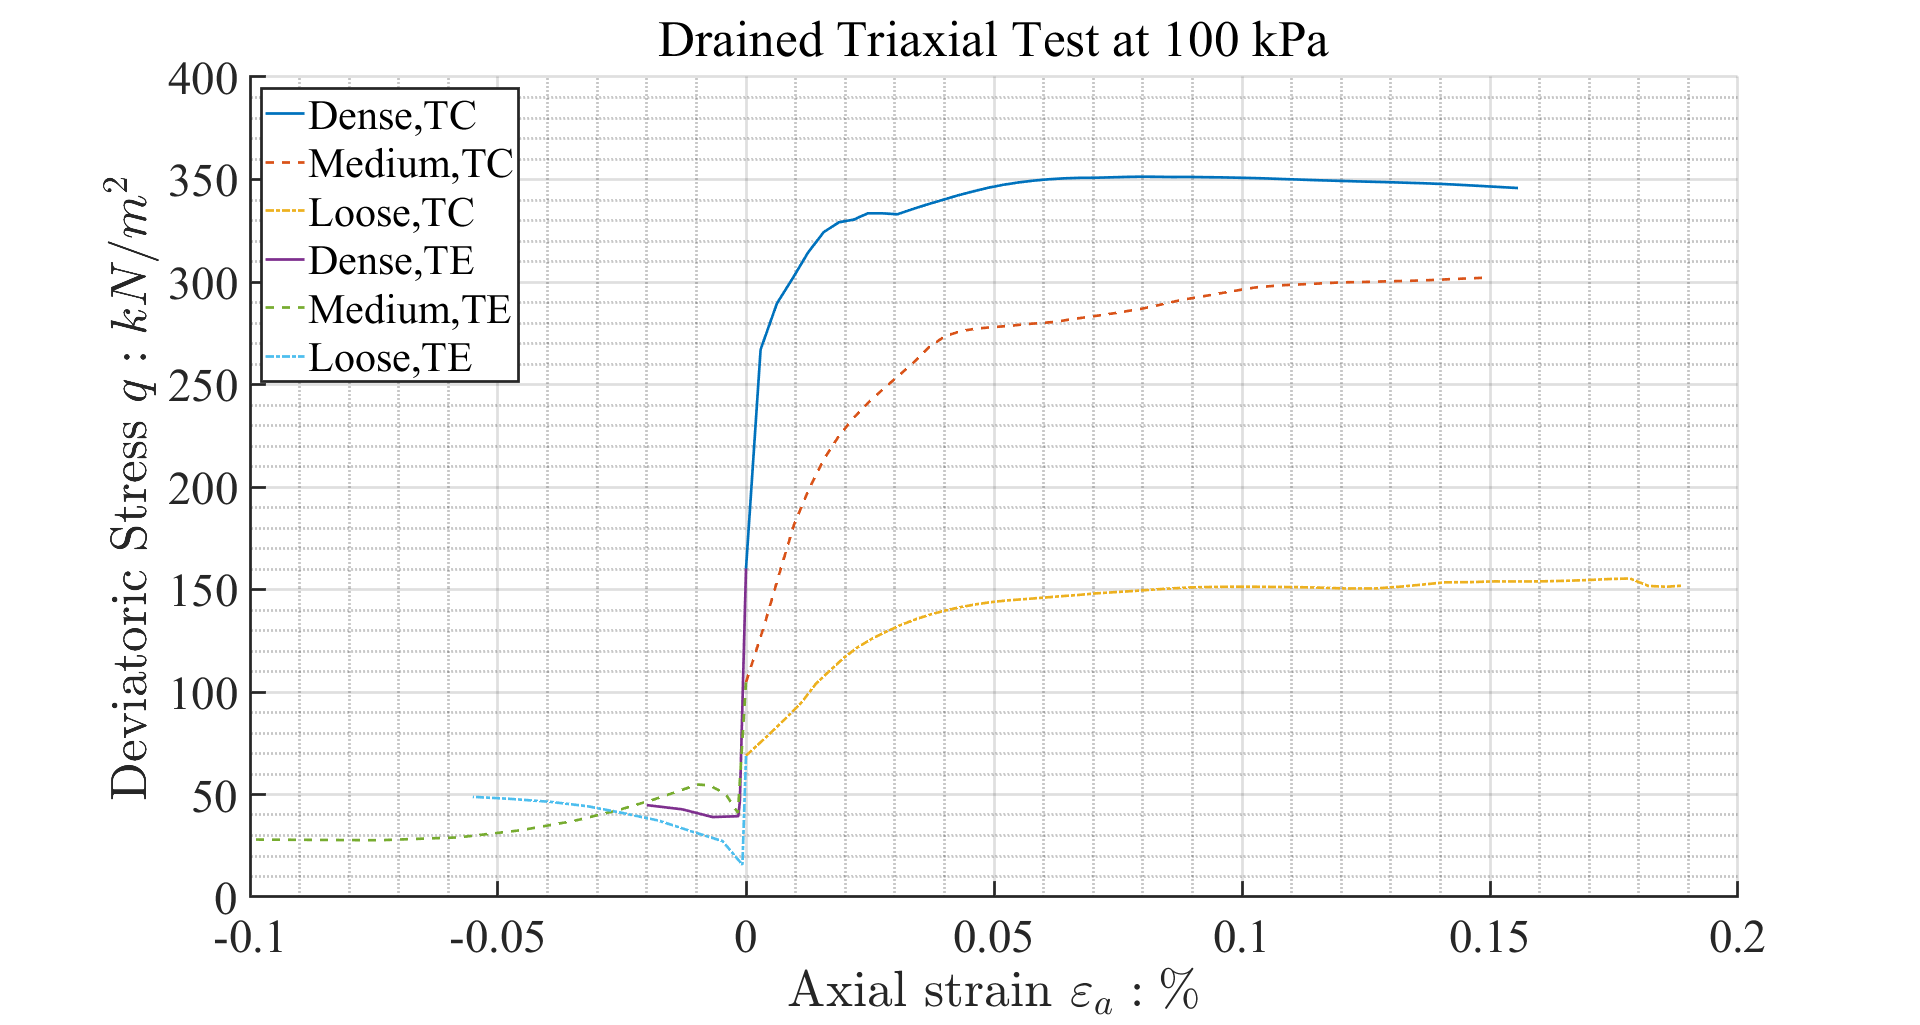
\includegraphics[width=1\linewidth]{myfigureeeeee/100} \caption{Result of Drained Triaxial test at 100 kPa}\label{fig:unnamed-chunk-11}
\end{figure}

\hypertarget{result-of-elemental-triaxial-test-at-200-kpa}{%
\subsubsection{Result of Elemental Triaxial Test at 200 kPa}\label{result-of-elemental-triaxial-test-at-200-kpa}}

Triaxial test at radial stress of 200 kPa is simulated using one by one block of the finite elmeent formulation with the EMC model.

\begin{figure}[H]
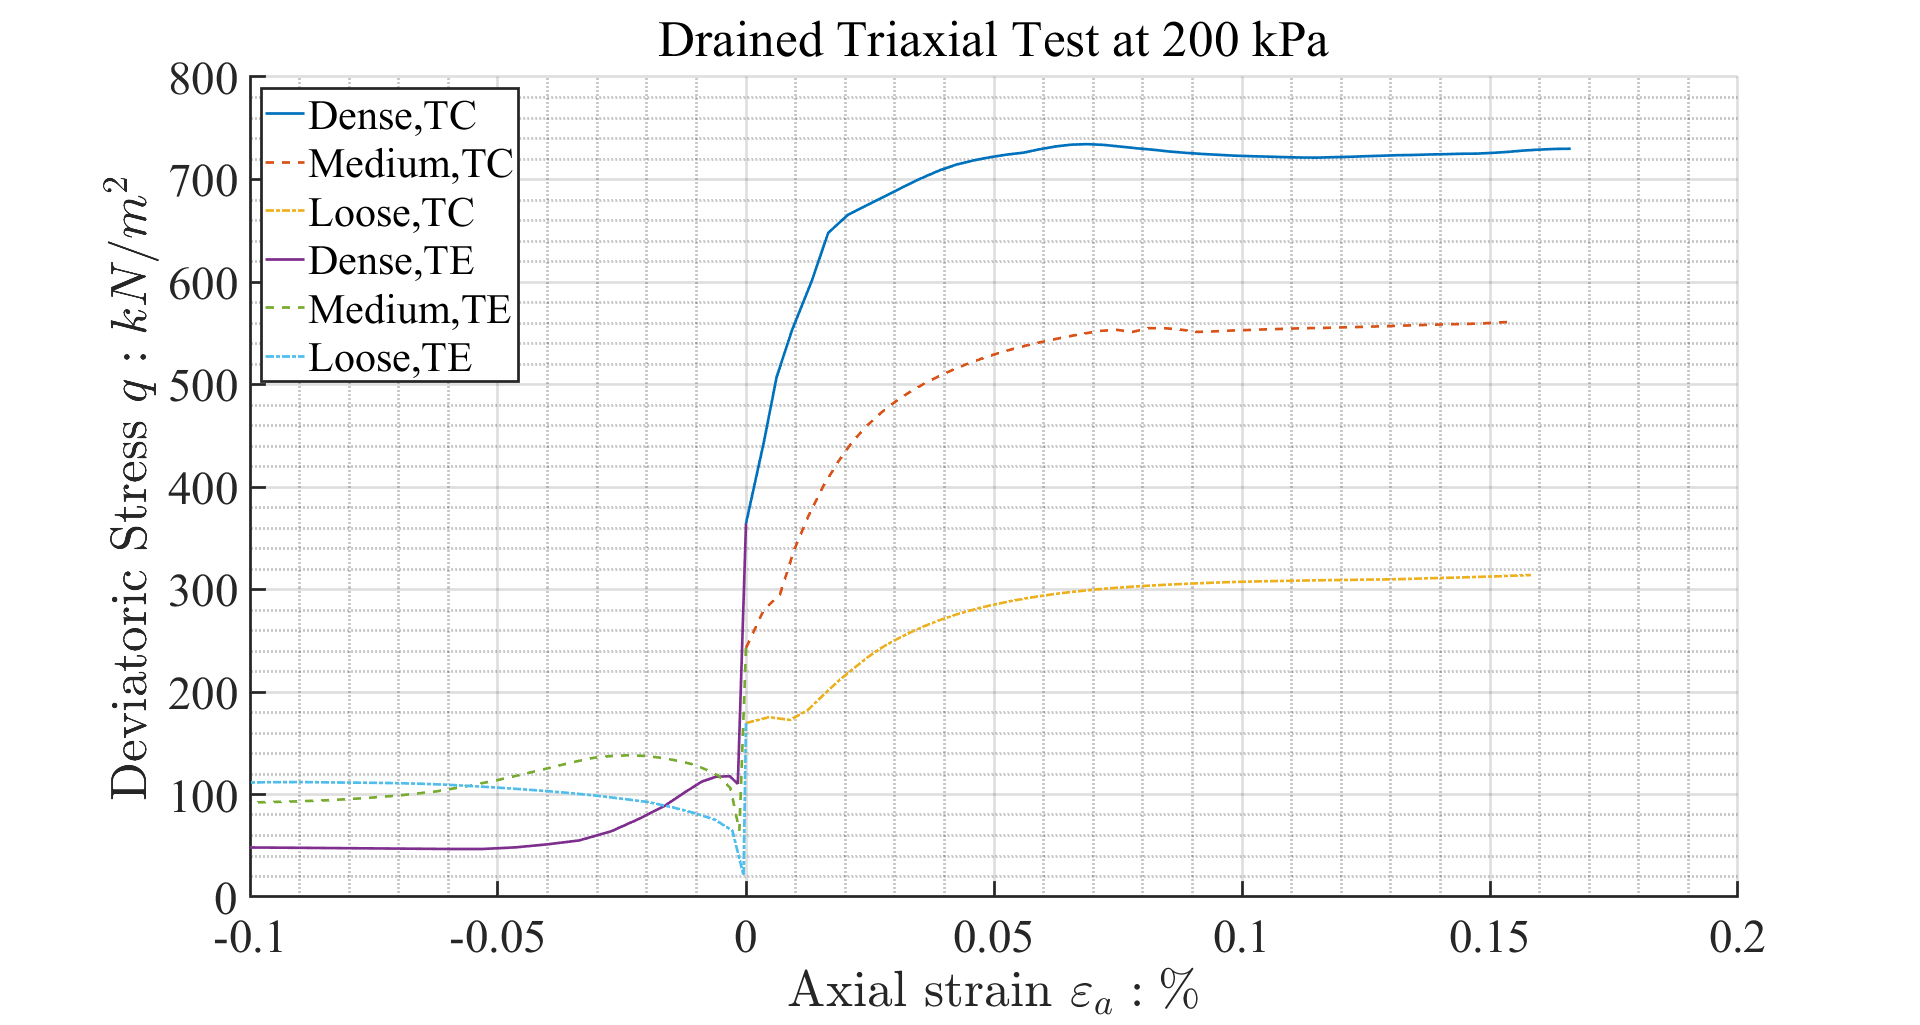
\includegraphics[width=1\linewidth]{myfigureeeeee/200} \caption{Result of Drained Triaxial test at 200 kPa}\label{fig:unnamed-chunk-12}
\end{figure}

\hypertarget{soil-parameters-1}{%
\section{Soil Parameters}\label{soil-parameters-1}}

\hypertarget{strainsoftening-stiffnesshardening-model-1}{%
\subsection{Strain---Softening Stiffness---Hardening Model}\label{strainsoftening-stiffnesshardening-model-1}}

Here is a table presenting the model parameters used by Sakai and Tanaka (1993).

\begin{table}[H]
\centering
{%
\begin{tabular}{@{}llll@{}}
\toprule
Parameters                                       & Loose & Medium & Dense \\ \midrule
Density $\gamma (kN/m3)$                       & 13.5  & 14.8   & 16.3  \\
Void ratio $e$                                   & 0.95  & 0.78   & 0.62  \\
Relative density $D_r$                           & 0.05  & 0.53   & 0.95  \\
Coefficient of shear modulus, $G_0$              & 500   & 500    & 500   \\
Poisson's ratio, $\nu$                           & 0.3   & 0.3    & 0.3   \\
Peak friction angle, $\phi_p (^{\circ})$       & 33    & 38     & 45    \\
Residual friction angle, $\phi_r (^{\circ})$   & 33    & 33     & 33    \\
Dilation angle, $\psi (^{\circ})$              & 0     & 10     & 20    \\
Shear band thickness, $S.B. (cm)$                & 0.3   & 0.3    & 0.3   \\
Soil parameter, $a$                              & 0.1   & 0.1    & 0.1   \\
Soil parameter, $b$                              & 0.8   & 0.4    & 0.1   \\
Soil parameter, $\varepsilon_d$                 & 0.3   & 0.3    & 0.3   \\
Soil parameter, $m$                              & 0.4   & 0.2    & 0.1   \\
Soil parameter, $\beta$                          & 0.1   & 0.1    & 0.1   \\ \bottomrule
\end{tabular}%
}
\caption{Model parameters used by Sakai and Tanaka, 1993}
\label{tab: model parameters used by Sakai and Tanaka, 1993}
\end{table}

\hypertarget{nonassociated-flow-rule-na-1}{%
\subsection{Nonassociated Flow Rule (NA)}\label{nonassociated-flow-rule-na-1}}

Here is a table presenting the model parameters used in Nonassociated (NA) simulations.

\begin{table}[H]
\centering
{%
\begin{tabular}{@{}llll@{}}
\toprule
Parameter                    & Dense       & Medium      & Loose     \\ \midrule
$E (MPa)$                    & 50          & 25          & 15        \\
$\nu$                        & 0.3         & 0.25        & 0.2       \\
$c (kPa)$                    & 0           & 0           & 0         \\
$\phi(^{\circ})$             & 40          & 35          & 30        \\
$\psi(^{\circ})$             & 10          & 5           & 0         \\
$\gamma_{dry}(kN/m^3)$       & 18          & 16          & 14        \\
$\gamma_{sat}(kN/m^3)$       & 21          & 20          & 19        \\
$K_0$                        & 0.3572      & 0.4264      & 0.5       \\ \bottomrule
\end{tabular}%
}
\caption{Soil parameters used in nonassociated flow (NA) simulations}
\label{tab:Soil parameters used in nonassociated flow NA simulations}
\end{table}

\hypertarget{extended-mohrcoulomb-model-emc-1}{%
\subsection{Extended Mohr---Coulomb Model (EMC)}\label{extended-mohrcoulomb-model-emc-1}}

Here is a table presenting the model parameters used in Extended Mohr-Coulomb (EMC) simulations.

\begin{table}[H]
\centering
{%
\begin{tabular}{@{}llll@{}}
\toprule
Parameter               & Dense   & Medium  & Loose  \\ \midrule
$E_{50} (MPa)$          & 50      & 25      & 13     \\
$E_{ur} (MPa)$          & 150     & 75      & 39     \\
$\nu_{ur}$              & 0.4     & 0.35    & 0.3    \\
$c (kPa)$               & 0       & 0       & 0      \\
$\phi(^{\circ})$        & 41      & 37      & 27     \\
$\psi(^{\circ})$        & 17      & 11      & -4     \\
$\gamma_{dry}(kN/m^3)$  & 18      & 16      & 14     \\
$\gamma_{sat}(kN/m^3)$  & 21      & 20      & 19     \\
$K_0$                   & 0.3572  & 0.4264  & 0.5    \\
$p_{ref} (kPa)$         & 100     & 100     & 100    \\
Soil parameter, m       & 0.5     & 0.5     & 0.5    \\ \bottomrule
\end{tabular}%
}
\caption{Soil parameters used in Extended Mohr-Coulomb Model (EMC)simulations}
\label{tab:Soil parameters used in Extended Mohr-Coulomb Model simulations}
\end{table}

\hypertarget{convergence-criteria}{%
\section{Convergence Criteria}\label{convergence-criteria}}

\hypertarget{mesh-convergence}{%
\subsection{Mesh Convergence}\label{mesh-convergence}}

Here is a table presenting the result of mesh convergence test on both NA and EMC models.\\
The goal of the mesh convergence test usually is to seek the acceptable range of number of the mesh size.
However, the interest in the present paper differs from the previously investigated objectives, in a way that the object sought is not the same.\\
The present paper seeks to draw a more detailed analysis of the failure surface formed as the soil is sheared.\\
Some authors in the past described this with the width of the shear band (Tanaka and Sakai, 1993). However, the present paper deals only with the limit analysis formulation using the Extended Mohr-Coulomb model.

\begin{table}[H]
\centering
{%
\begin{tabular}{@{}lllll@{}}
\toprule
Type of Analysis           & Mesh Number & $p_u,kN/m2$ & Variance & Std  \\ \midrule
Non-associated $(NA)$        & 250         & 137.7       & 0.11     & 0.33 \\
Non-associated $(NA)$        & 500         & 135.8       & 1.23     & 1.11 \\
Non-associated $(NA)$        & 1000        & 129.4       & 13.85    & 3.72 \\
Non-associated $(NA)$        & 2000        & 139.8       & 0.28     & 0.52 \\
Non-associated $(NA)$        & 5000        & 138.2       & 0.02     & 0.13 \\
Non-associated $(NA)$        & 10000       & 141.7       & 1.69     & 1.30 \\
Non-associated $(NA)$        & 20000       & 147         & 12.00    & 3.46 \\
Extened Mohr-Coulomb $(EMC)$ & 250         & 161.3       & 1.51     & 1.23 \\
Extened Mohr-Coulomb $(EMC)$ & 500         & 159.6       & 0.29     & 0.54 \\
Extened Mohr-Coulomb $(EMC)$ & 1000        & 161.4       & 1.62     & 1.27 \\
Extened Mohr-Coulomb $(EMC)$ & 2000        & 158.4       & 0.00     & 0.05 \\
Extened Mohr-Coulomb $(EMC)$ & 5000        & 157.3       & 0.16     & 0.40 \\
Extened Mohr-Coulomb $(EMC)$ & 10000       & 156.2       & 0.73     & 0.85 \\
Extened Mohr-Coulomb $(EMC)$ & 20000       & 153.8       & 3.35     & 1.83 \\ \bottomrule
\end{tabular}%
}
\caption{Setup and result of mesh convergence test}
\label{tab:Setup and result of mesh convergence test}
\end{table}

\hypertarget{mesh-convergence-results}{%
\subsubsection{Mesh Convergence Results}\label{mesh-convergence-results}}

The reulst of the present investigation is the determination of the number of the mesh elements be around 2000.\\
However, it is noted that further studies, outside of this paper, is onto the maximum number of the elements to be studied, for this will enhance the visualization of the shear band formation, as well as the guidance onto the study of the shear dissipation.

\begin{figure}[H]
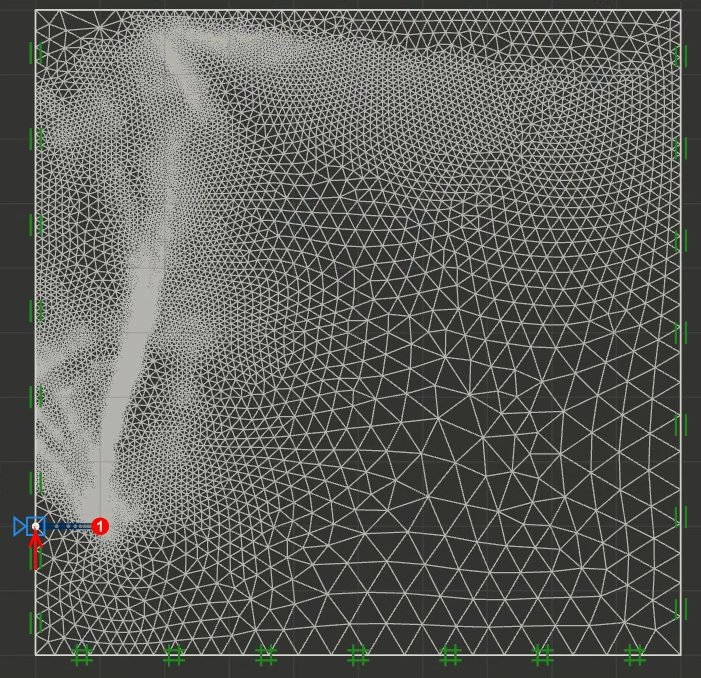
\includegraphics[width=1\linewidth]{myfigureeeeee/20000} \caption{Typical result from mesh convergence test (maximum number of elements)}\label{fig:unnamed-chunk-13}
\end{figure}

\begin{figure}[H]
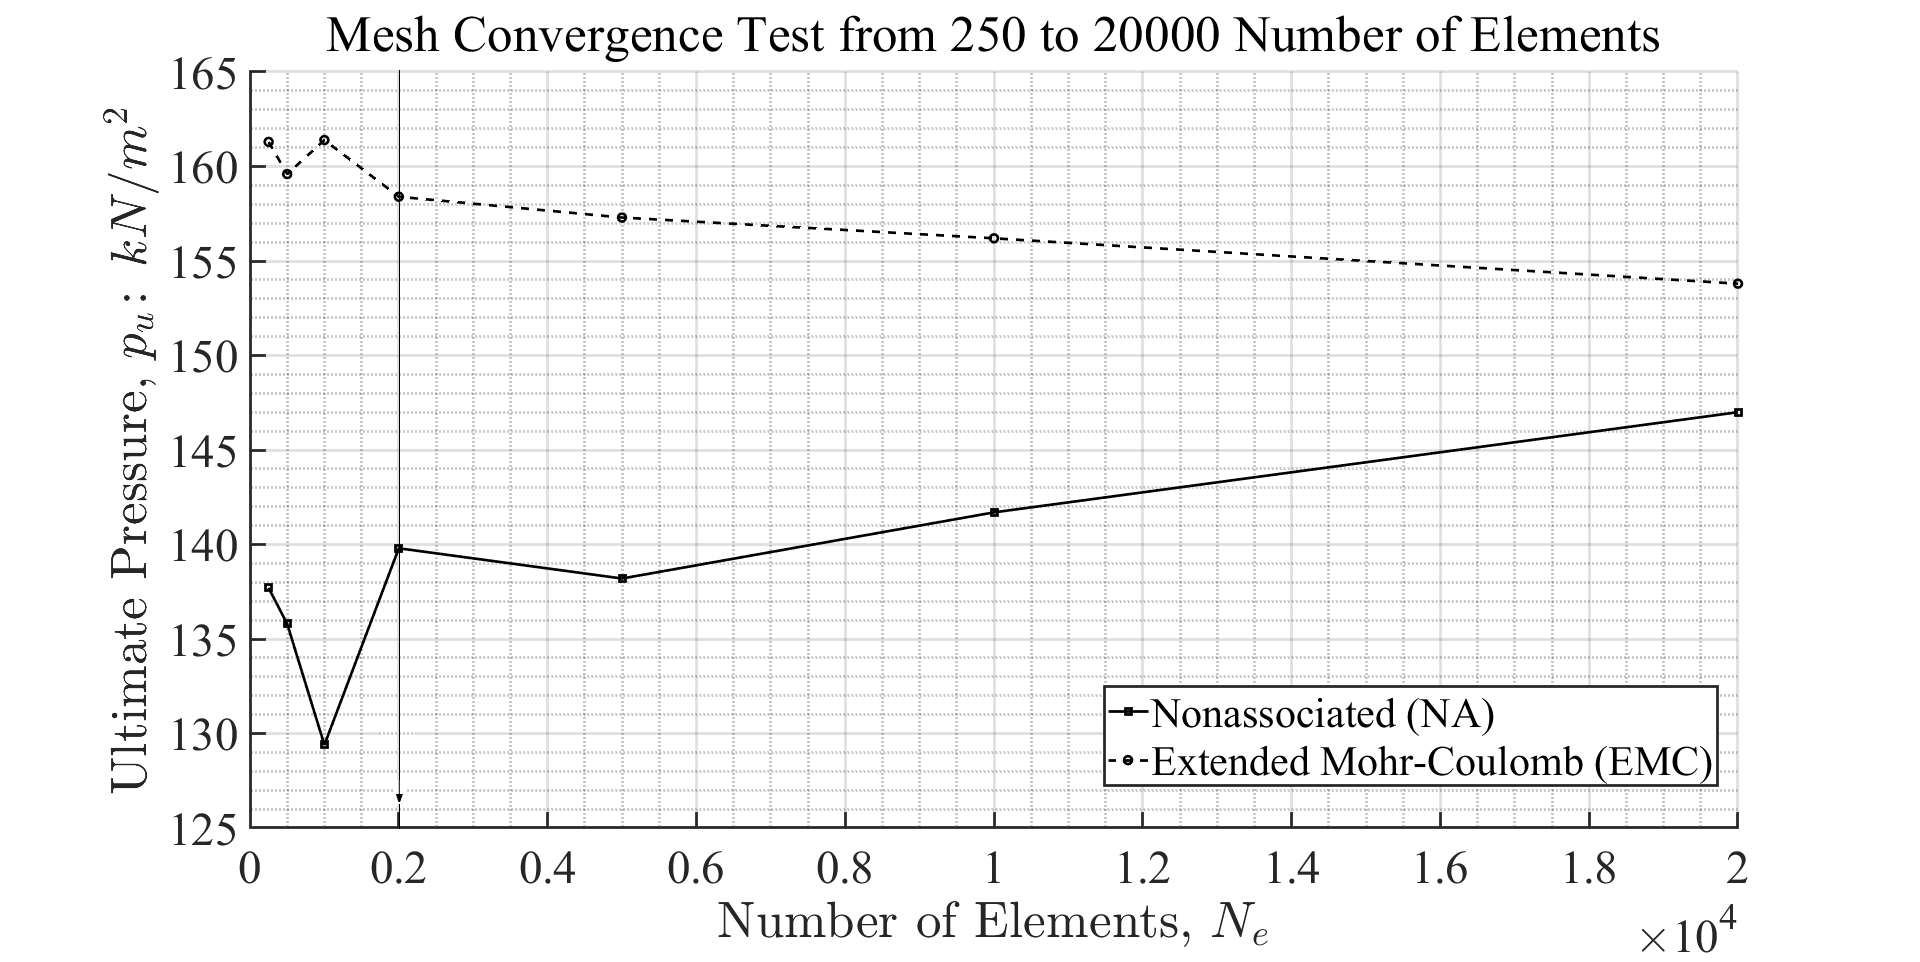
\includegraphics[width=1\linewidth]{myfigureeeeee/meshresult} \caption{Result of the mesh convergence test, which confirms that about 2000 elements are acceptable}\label{fig:unnamed-chunk-14}
\end{figure}

\begin{figure}[H]
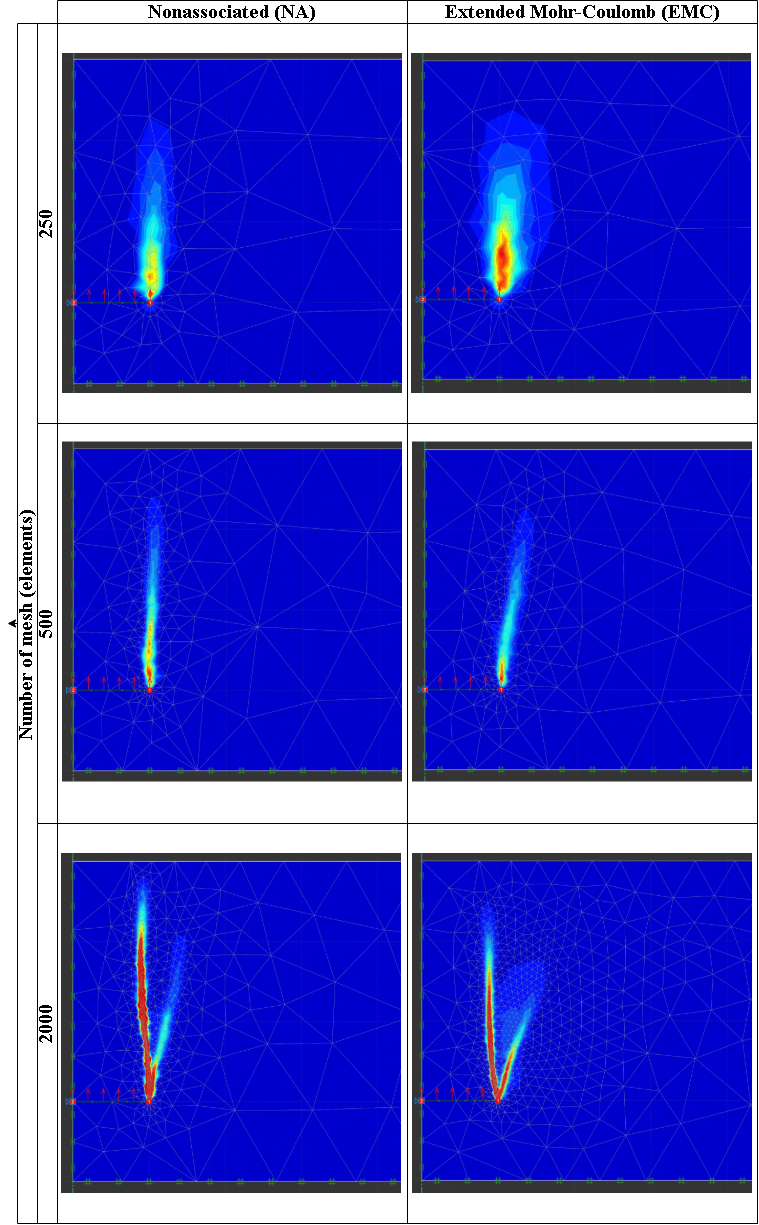
\includegraphics[width=1\linewidth]{myfigureeeeee/1} \caption{Shear Dissipation of the mesh convergence test of 250, 500, 2000 elements}\label{fig:unnamed-chunk-15}
\end{figure}

\begin{figure}[H]
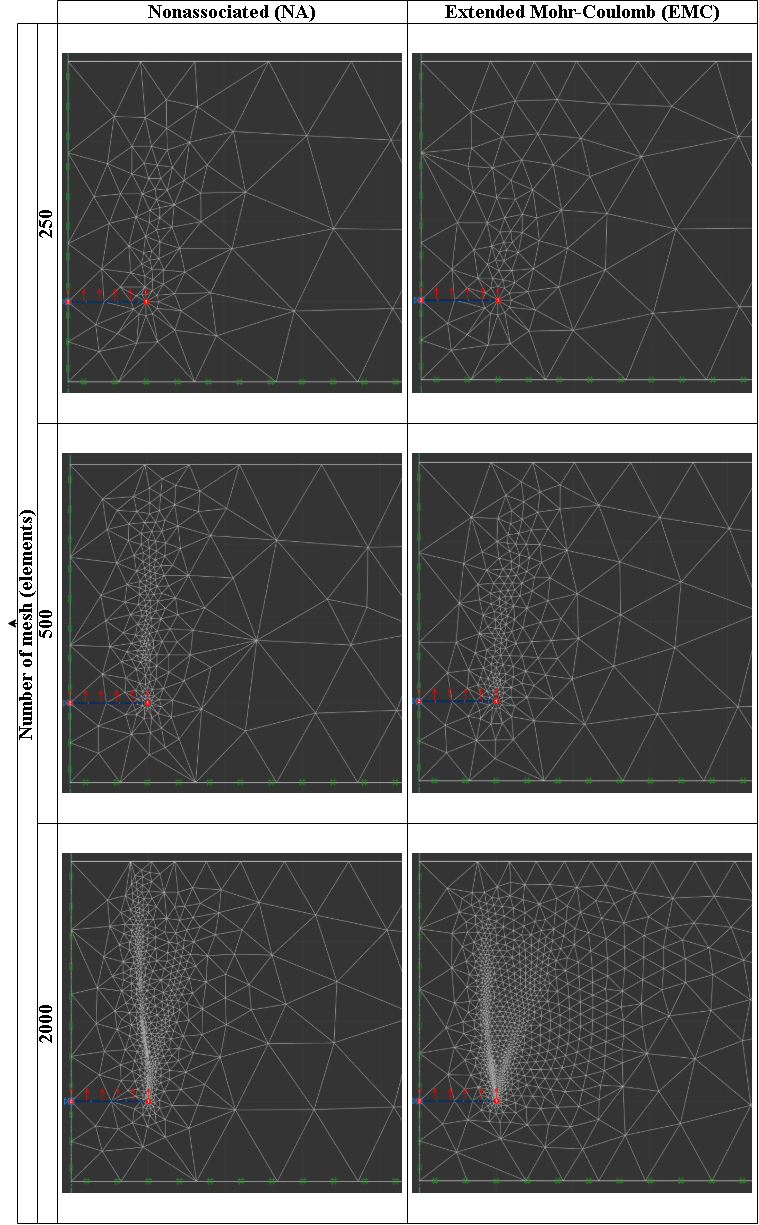
\includegraphics[width=1\linewidth]{myfigureeeeee/4} \caption{Mesh of 250, 500, 2000 elements}\label{fig:unnamed-chunk-16}
\end{figure}

\begin{figure}[H]
\includegraphics[width=1\linewidth]{myfigureeeeee/2} \caption{Shear Dissipation of the mesh convergence test of 5000, 10000, 20000 elements}\label{fig:unnamed-chunk-17}
\end{figure}

\begin{figure}[H]
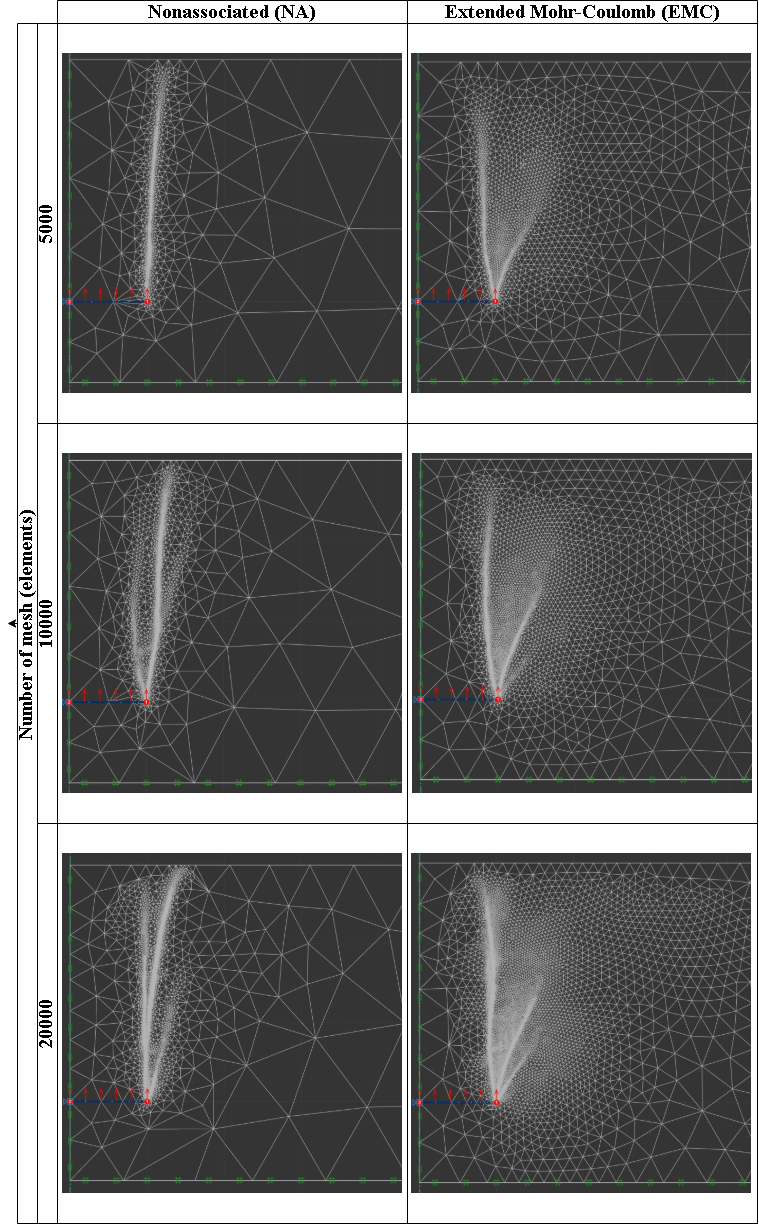
\includegraphics[width=1\linewidth]{myfigureeeeee/3} \caption{Mesh of 5000, 10000, 20000 elements}\label{fig:unnamed-chunk-18}
\end{figure}

\hypertarget{boundary-convergence}{%
\subsection{Boundary Convergence}\label{boundary-convergence}}

The soil tank width and the distance below the anchor to the soil tank boundary are the primary condern for the modeling.\\
Therefore, the optimized value of the soil tank width has been investigated, by differing the values from 10B to 3B, , wherein B refers to the width of the anchor plate.

\begin{figure}[H]
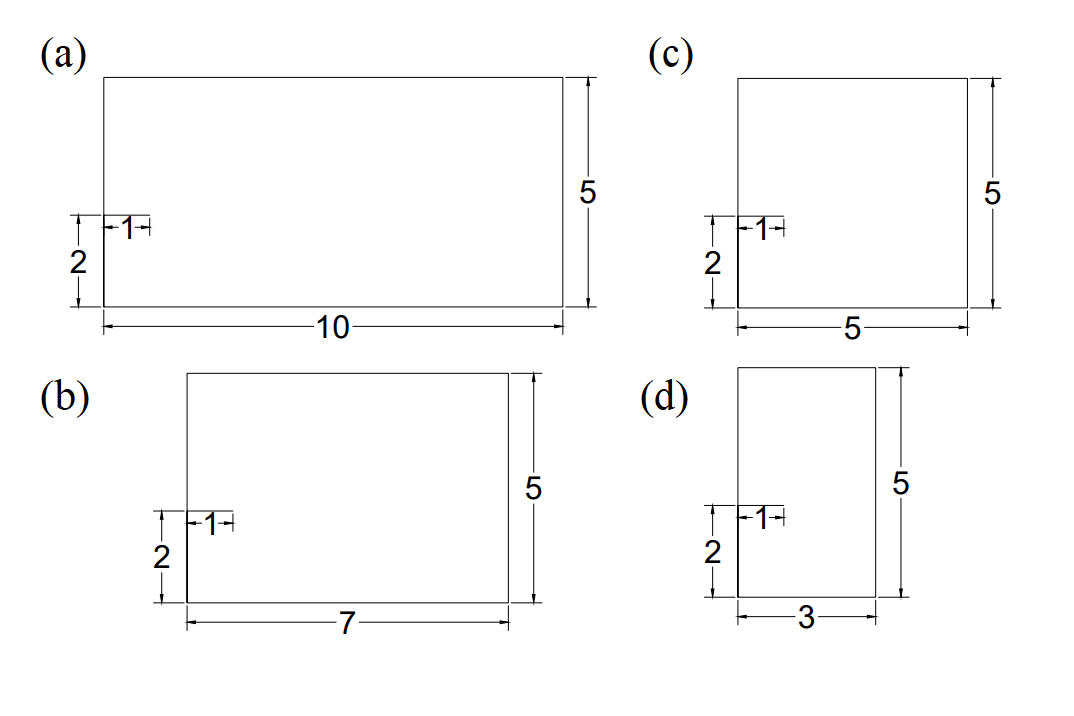
\includegraphics[width=1\linewidth]{myfigureeeeee/boundary} \caption{Convergence test setup on different boundary size: (a) 10B, (b) 7B, (c) 5B, (d) 3B}\label{fig:unnamed-chunk-19}
\end{figure}

Due to the reasoning which considers the method of mesh adaptivity, insignificant effect onto the extension of the soil tank width has been deemed acceptable by the author. Therefore, the result of the boundary convergence test is determined at 10B.

\begin{figure}[H]
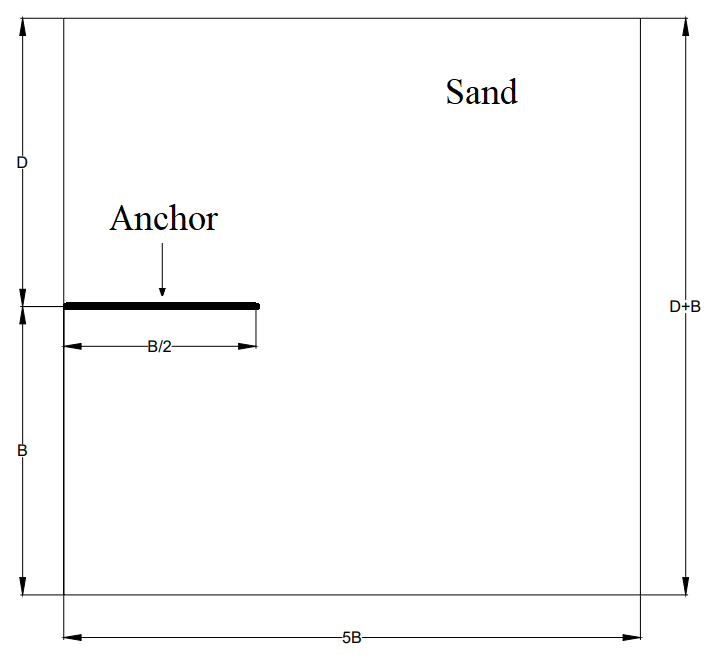
\includegraphics[width=1\linewidth]{myfigureeeeee/boundary convergence2} \caption{Final boundary decision schematic for numerical simulations}\label{fig:unnamed-chunk-20}
\end{figure}

Here is a table presenting the setup of boundary convergence test on both NA and EMC models.

\begin{table}[H]
\centering
{%
\begin{tabular}{@{}llllllll@{}}
\toprule
Width Boundary & Depth Below Anchor & D/B & Soil Type & Test Type \\ \midrule
10B            & 2B                 & 3   & Dense     & NA, EMC   \\
7B             & 2B                 & 3   & Dense     & NA, EMC   \\
5B             & 2B                 & 3   & Dense     & NA, EMC   \\
3B             & 2B                 & 3   & Dense     & NA, EMC   \\
10B            & 2B                 & 3   & Medum     & NA, EMC   \\
7B             & 2B                 & 3   & Medum     & NA, EMC   \\
5B             & 2B                 & 3   & Medum     & NA, EMC   \\
3B             & 2B                 & 3   & Medum     & NA, EMC   \\
10B            & 2B                 & 3   & Loose     & NA, EMC   \\
7B             & 2B                 & 3   & Loose     & NA, EMC   \\
5B             & 2B                 & 3   & Loose     & NA, EMC   \\
3B             & 2B                 & 3   & Loose     & NA, EMC   \\ \bottomrule

\end{tabular}%
}
\caption{Setup of boundary convergence test}
\label{tab:Setup of boundary convergence test}
\end{table}

\hypertarget{boundary-convergence-results}{%
\subsubsection{Boundary Convergence Results}\label{boundary-convergence-results}}

\hypertarget{result}{%
\chapter{Results}\label{result}}

\chaptermark{Result}

\minitoc 

\hypertarget{parametric-study}{%
\section{Parametric Study}\label{parametric-study}}

Here is a table presenting the setup of the numerical simulations on both NA and EMC models.\\
The code refers to the differing width of the plate anchor, , whereas the number specifies if its embedment ratio is either 1, 2, or 3.

\begin{longtable}[c]{cccrrr}
\caption{Setup for numerical simulations}
\label{tab:Setup for numerical simulations}\\
\textbf{Code} & \textbf{Test No.} & \textbf{Density} & \multicolumn{1}{c}{\textbf{B, mm}} & \multicolumn{1}{c}{\textbf{D, mm}} & \multicolumn{1}{c}{\textbf{D/B}} \\
\endfirsthead
%
\multicolumn{6}{c}%
{{\bfseries Table \thetable\ continued from previous page}} \\
\textbf{Code} & \textbf{Test No.} & \textbf{Density} & \multicolumn{1}{c}{\textbf{B, mm}} & \multicolumn{1}{c}{\textbf{D, mm}} & \multicolumn{1}{c}{\textbf{D/B}} \\
\endhead
%
A & LA1 & Loose  & 40   & 40    & 1 \\
B & LB1 & Loose  & 200  & 200   & 1 \\
C & LC1 & Loose  & 1000 & 1000  & 1 \\
D & LD1 & Loose  & 3500 & 3500  & 1 \\
E & LE1 & Loose  & 4500 & 4500  & 1 \\
G & LG1 & Loose  & 6500 & 6500  & 1 \\
A & MA1 & Medium & 40   & 40    & 1 \\
B & MB1 & Medium & 200  & 200   & 1 \\
C & MC1 & Medium & 1000 & 1000  & 1 \\
D & MD1 & Medium & 3500 & 3500  & 1 \\
E & ME1 & Medium & 4500 & 4500  & 1 \\
G & MG1 & Medium & 6500 & 6500  & 1 \\
A & DA1 & Dense  & 40   & 40    & 1 \\
B & DB1 & Dense  & 200  & 200   & 1 \\
C & DC1 & Dense  & 1000 & 1000  & 1 \\
D & DD1 & Dense  & 3500 & 3500  & 1 \\
E & DE1 & Dense  & 4500 & 4500  & 1 \\
G & DG1 & Dense  & 6500 & 6500  & 1 \\
A & LA2 & Loose  & 40   & 80    & 2 \\
B & LB2 & Loose  & 200  & 400   & 2 \\
C & LC2 & Loose  & 1000 & 2000  & 2 \\
D & LD2 & Loose  & 3500 & 7000  & 2 \\
E & LE2 & Loose  & 4500 & 9000  & 2 \\
G & LG2 & Loose  & 6500 & 13000 & 2 \\
A & MA2 & Medium & 40   & 80    & 2 \\
B & MB2 & Medium & 200  & 400   & 2 \\
C & MC2 & Medium & 1000 & 2000  & 2 \\
D & MD2 & Medium & 3500 & 7000  & 2 \\
E & ME2 & Medium & 4500 & 9000  & 2 \\
G & MG2 & Medium & 6500 & 13000 & 2 \\
A & DA2 & Dense  & 40   & 80    & 2 \\
B & DB2 & Dense  & 200  & 400   & 2 \\
C & DC2 & Dense  & 1000 & 2000  & 2 \\
D & DD2 & Dense  & 3500 & 7000  & 2 \\
E & DE2 & Dense  & 4500 & 9000  & 2 \\
G & DG2 & Dense  & 6500 & 13000 & 2 \\
A & LA3 & Loose  & 40   & 120   & 3 \\
B & LB3 & Loose  & 200  & 600   & 3 \\
C & LC3 & Loose  & 1000 & 3000  & 3 \\
D & LD3 & Loose  & 3500 & 10500 & 3 \\
E & LE3 & Loose  & 4500 & 13500 & 3 \\
G & LG3 & Loose  & 6500 & 19500 & 3 \\
A & MA3 & Medium & 40   & 120   & 3 \\
B & MB3 & Medium & 200  & 600   & 3 \\
C & MC3 & Medium & 1000 & 3000  & 3 \\
D & MD3 & Medium & 3500 & 10500 & 3 \\
E & ME3 & Medium & 4500 & 13500 & 3 \\
G & MG3 & Medium & 6500 & 19500 & 3 \\
A & DA3 & Dense  & 40   & 120   & 3 \\
B & DB3 & Dense  & 200  & 600   & 3 \\
C & DC3 & Dense  & 1000 & 3000  & 3 \\
D & DD3 & Dense  & 3500 & 10500 & 3 \\
E & DE3 & Dense  & 4500 & 13500 & 3 \\
G & DG3 & Dense  & 6500 & 19500 & 3
\end{longtable}

\hypertarget{effect-of-embedment-depth-ratio-fracdb}{%
\subsection{\texorpdfstring{Effect of Embedment Depth Ratio \(\frac{D}{B}\)}{Effect of Embedment Depth Ratio \textbackslash frac\{D\}\{B\}}}\label{effect-of-embedment-depth-ratio-fracdb}}

\hypertarget{overall-results-with-all-range-of-dense-medium-loose-sands}{%
\subsubsection{Overall Results with All Range of Dense, Medium, Loose Sands}\label{overall-results-with-all-range-of-dense-medium-loose-sands}}

\begin{figure}[H]
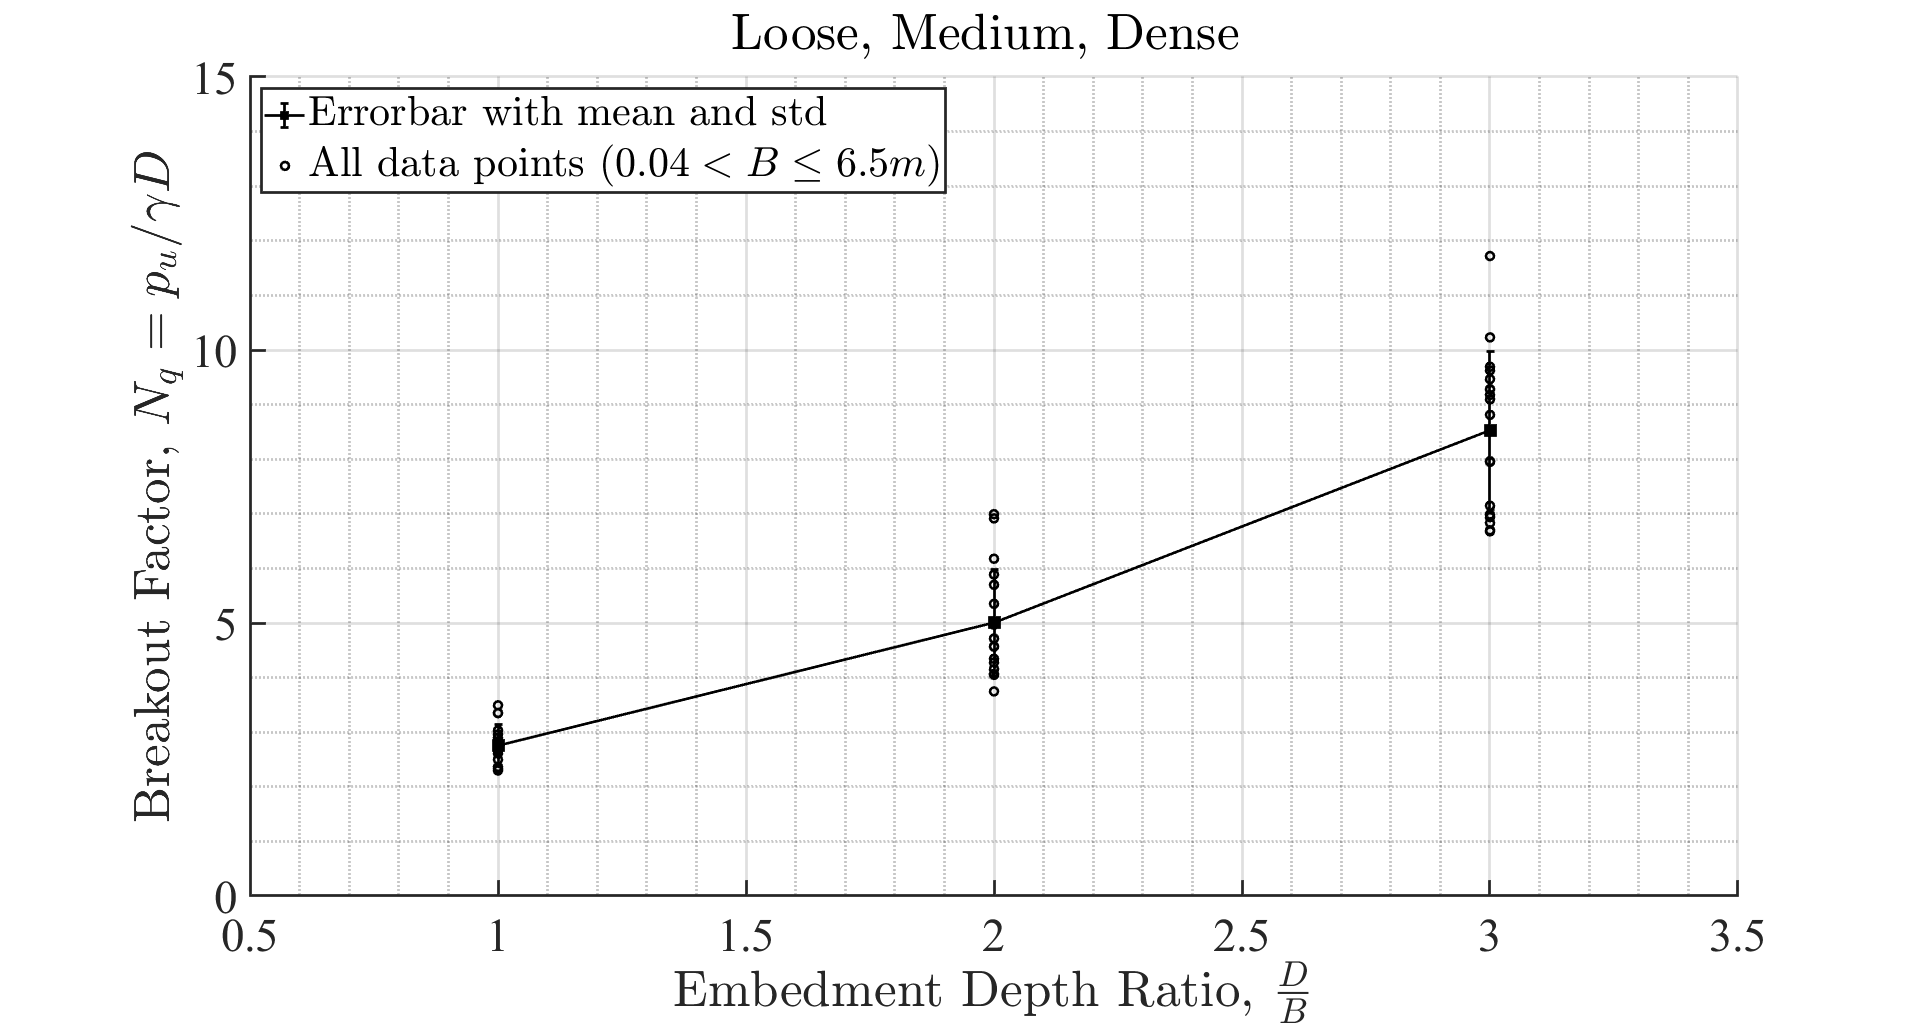
\includegraphics[width=1\linewidth]{myfigureeeeee/errorplot} \caption{Effect of embedment depth ratio on break-out factor for all densities of soil}\label{fig:unnamed-chunk-21}
\end{figure}

\hypertarget{for-different-sand-densities-loose-medium-dense}{%
\subsubsection{\texorpdfstring{For Different Sand Densities: \(Loose, Medium, Dense\)}{For Different Sand Densities: Loose, Medium, Dense}}\label{for-different-sand-densities-loose-medium-dense}}

\begin{figure}[H]
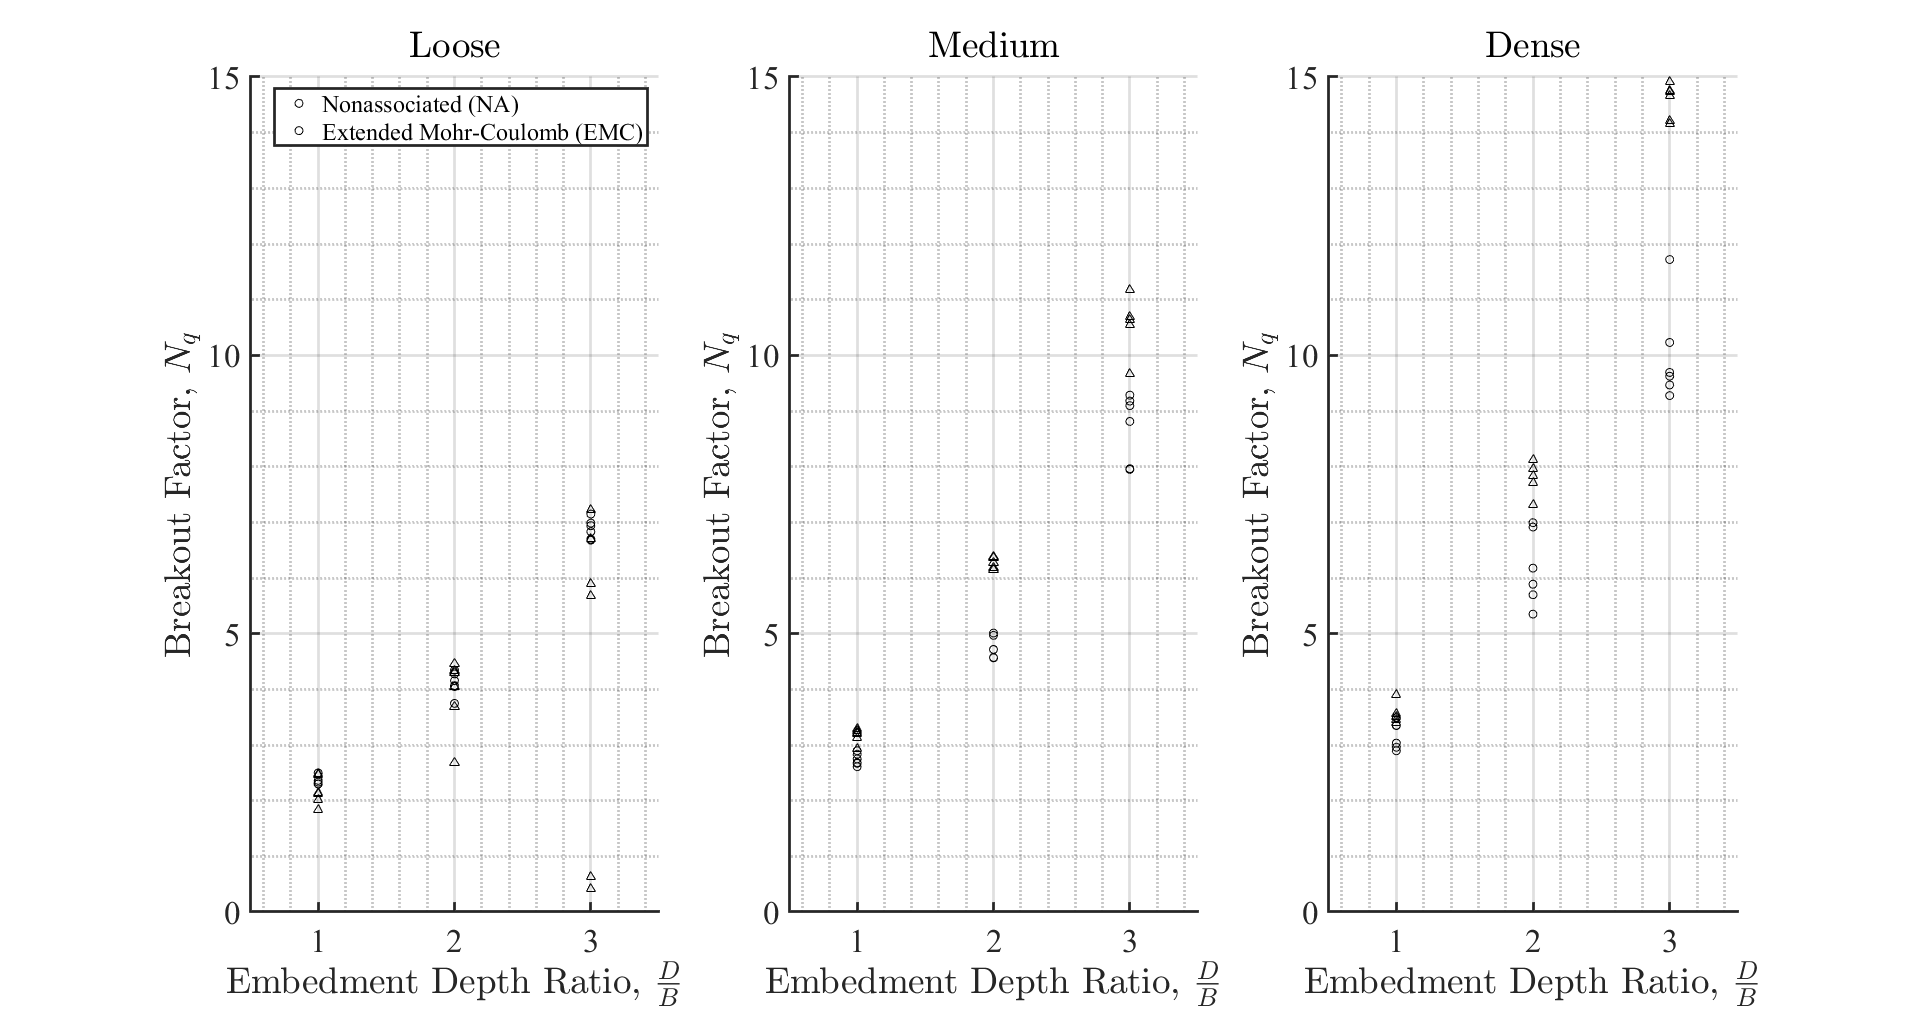
\includegraphics[width=1\linewidth]{myfigureeeeee/loosemediumdense} \caption{Effect of embedment depth ratio on break-out factor (a) loose (b) medium (c) dense}\label{fig:unnamed-chunk-22}
\end{figure}

\hypertarget{effect-of-width-b}{%
\subsection{\texorpdfstring{Effect of Width \(B\)}{Effect of Width B}}\label{effect-of-width-b}}

\hypertarget{overall-results-with-all-range-of-dense-medium-loose-sands-1}{%
\subsubsection{Overall Results with All Range of Dense, Medium, Loose Sands}\label{overall-results-with-all-range-of-dense-medium-loose-sands-1}}

\begin{figure}[H]
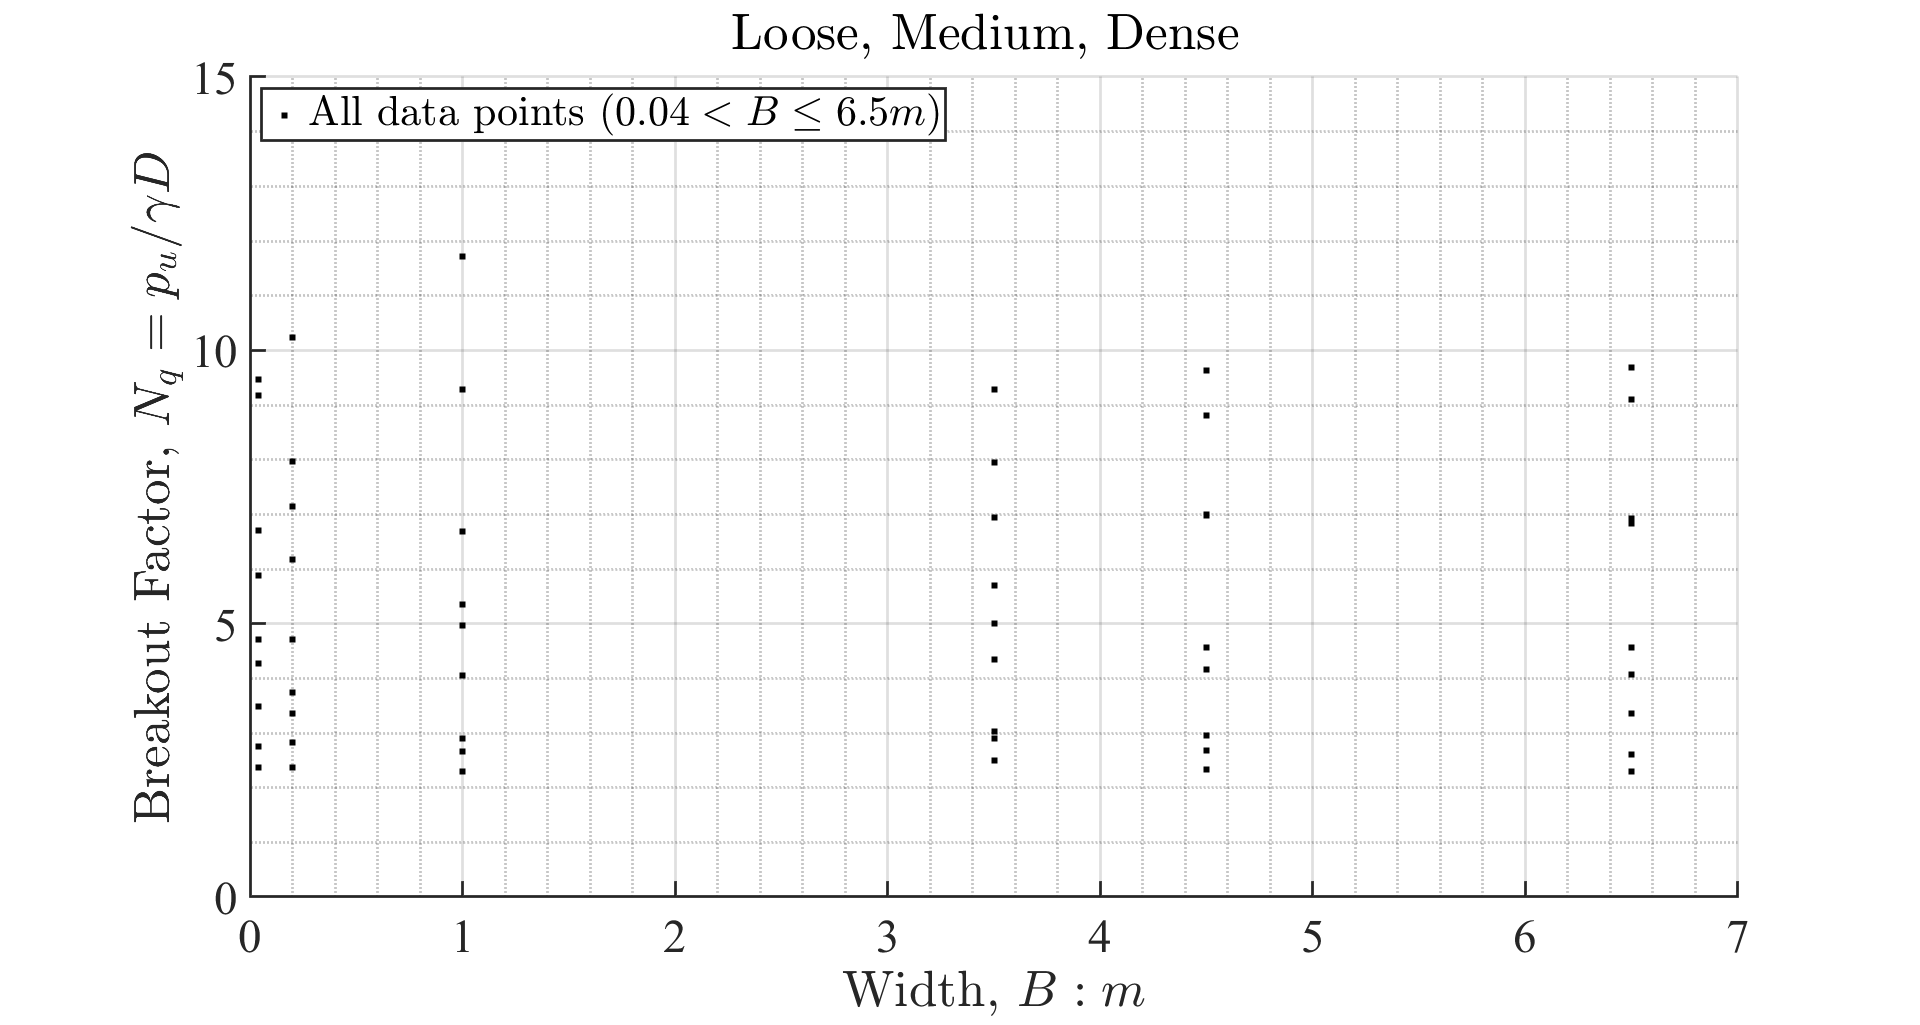
\includegraphics[width=1\linewidth]{myfigureeeeee/width_B} \caption{Effect of width of plate for all densities of soil}\label{fig:unnamed-chunk-23}
\end{figure}

\hypertarget{shear-dissipation}{%
\subsection{Shear Dissipation}\label{shear-dissipation}}

\begin{figure}[H]
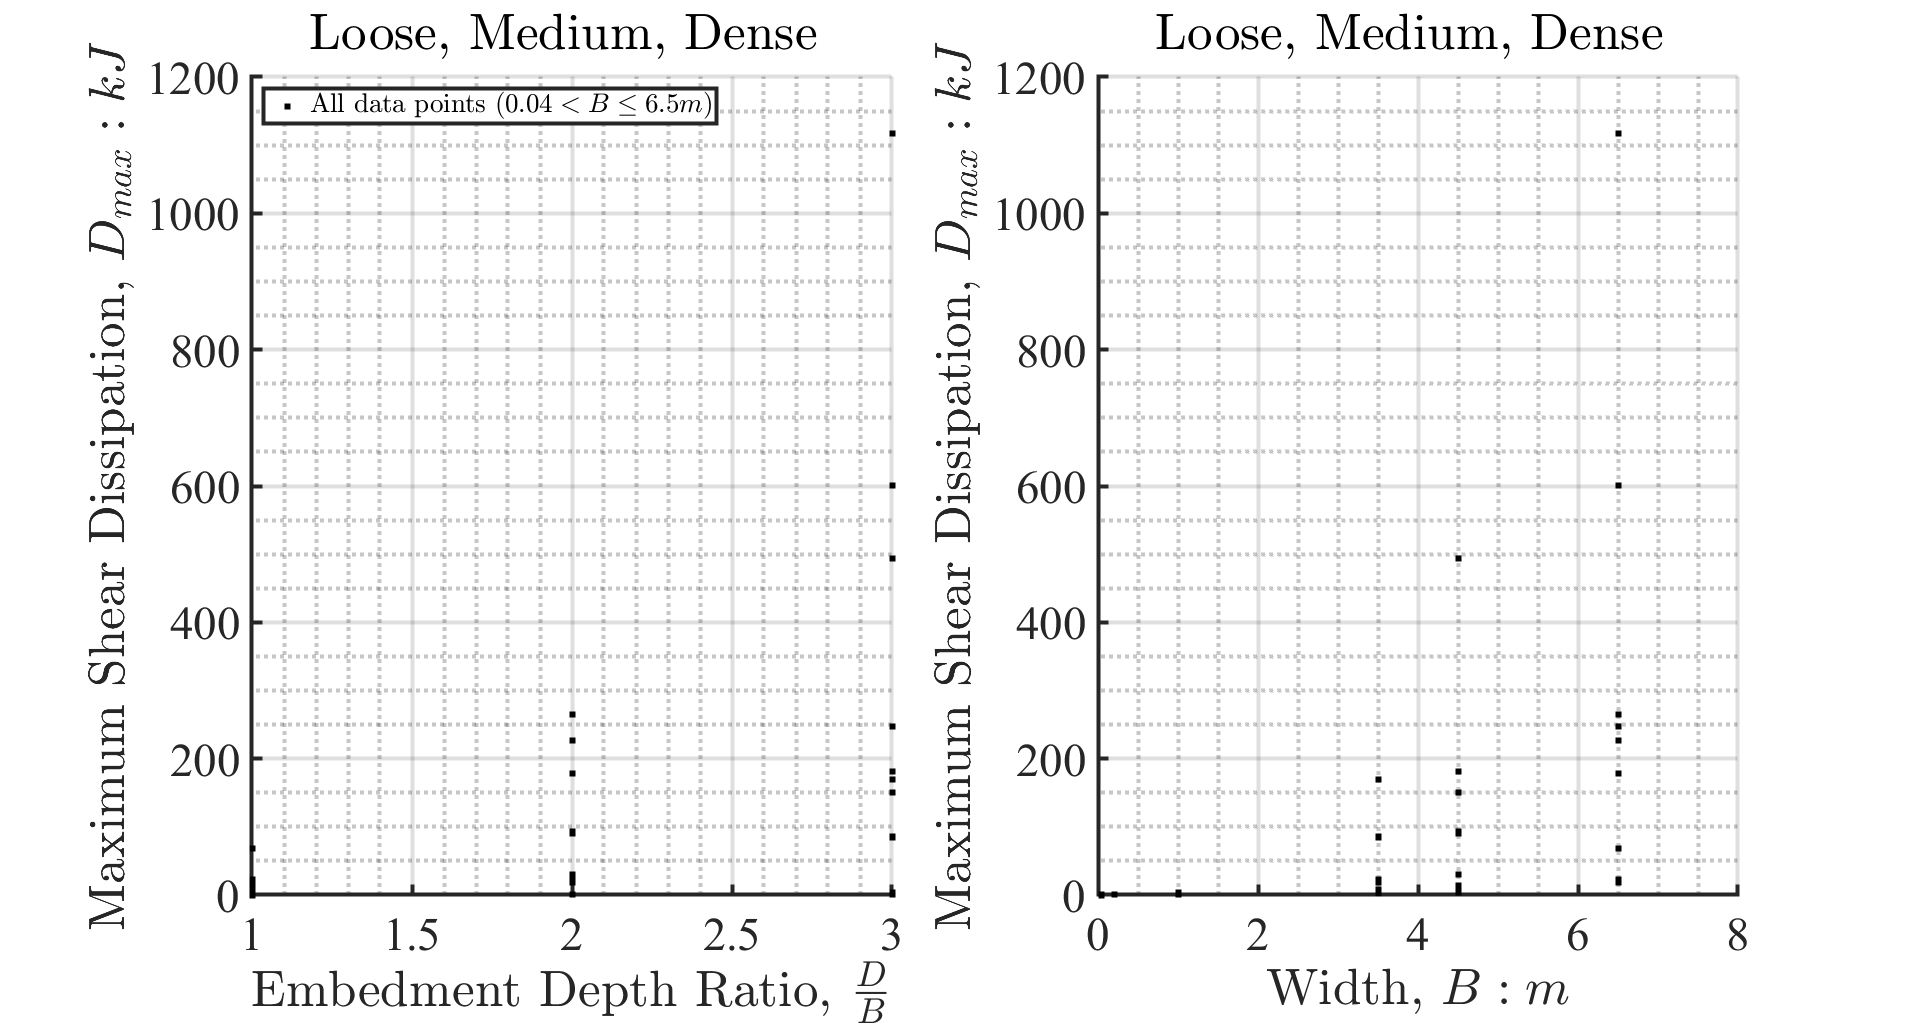
\includegraphics[width=1\linewidth]{myfigureeeeee/shear_dissipation_together} \caption{Effect of embedment depth and width on shear dissipation for all densities of soil}\label{fig:unnamed-chunk-24}
\end{figure}

\begin{figure}[H]
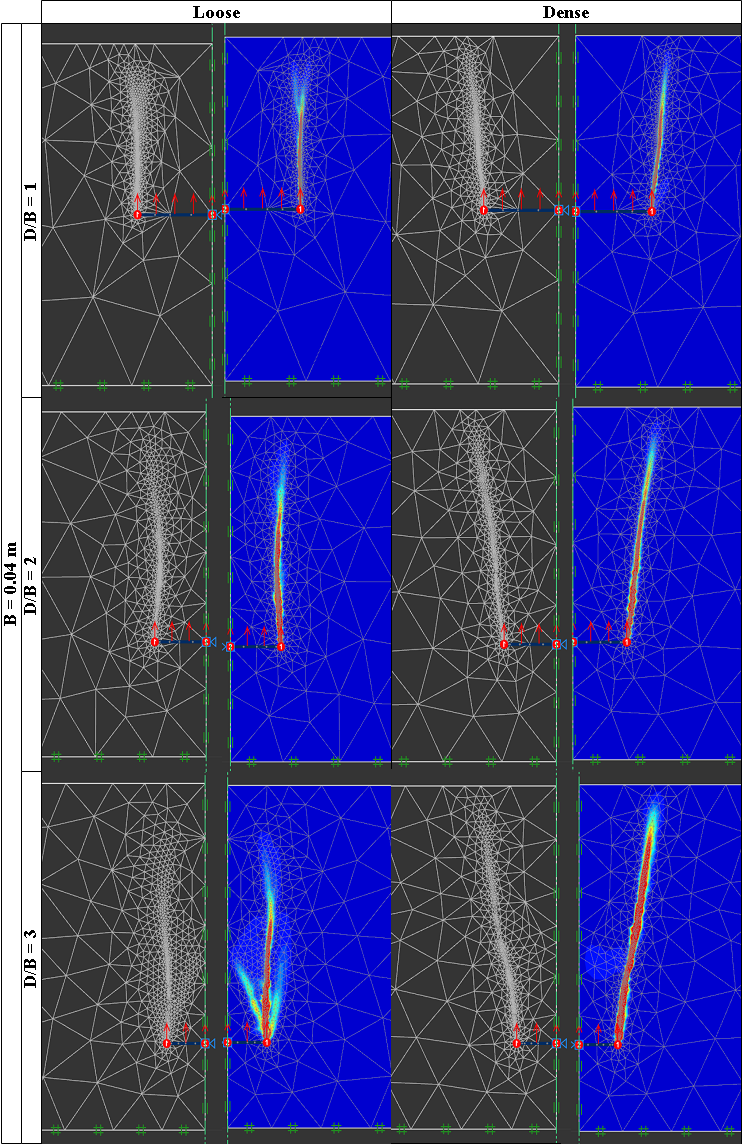
\includegraphics[width=1\linewidth]{myfigureeeeee/A_point_zero_four_meter} \caption{Shear dissipation of NA model at 10 percent of the maximum value and $B = 0.04m$}\label{fig:unnamed-chunk-25}
\end{figure}

\begin{figure}[H]
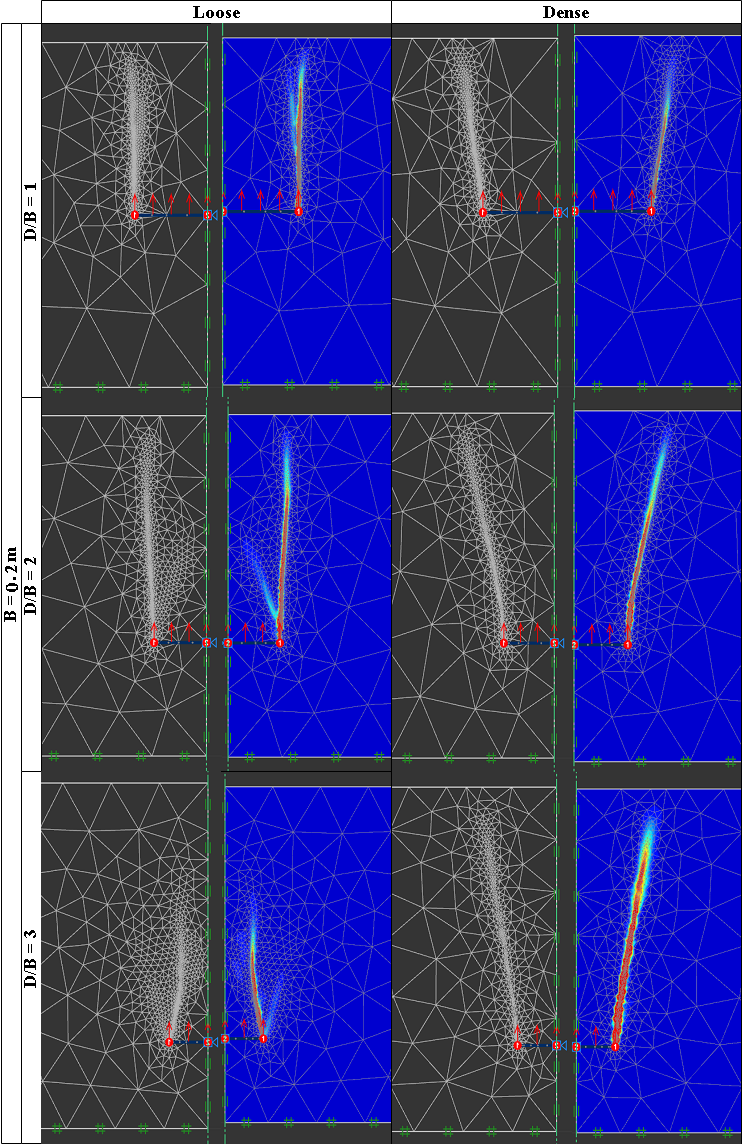
\includegraphics[width=1\linewidth]{myfigureeeeee/B_point_two_meter} \caption{Shear dissipation of NA model at 10 percent of the maximum value and $B = 0.2m$}\label{fig:unnamed-chunk-26}
\end{figure}

\begin{figure}[H]
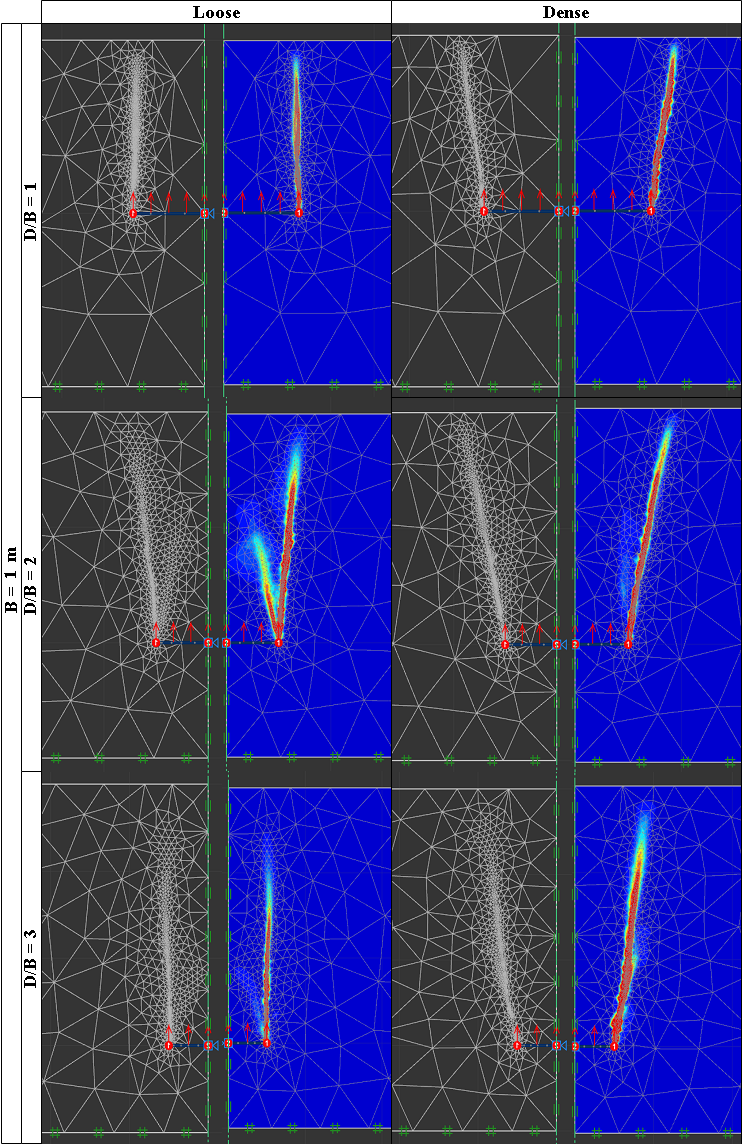
\includegraphics[width=1\linewidth]{myfigureeeeee/C_one_meter} \caption{Shear dissipation of NA model at 10 percent of the maximum value and $B = 1.0m$}\label{fig:unnamed-chunk-27}
\end{figure}

\begin{figure}[H]
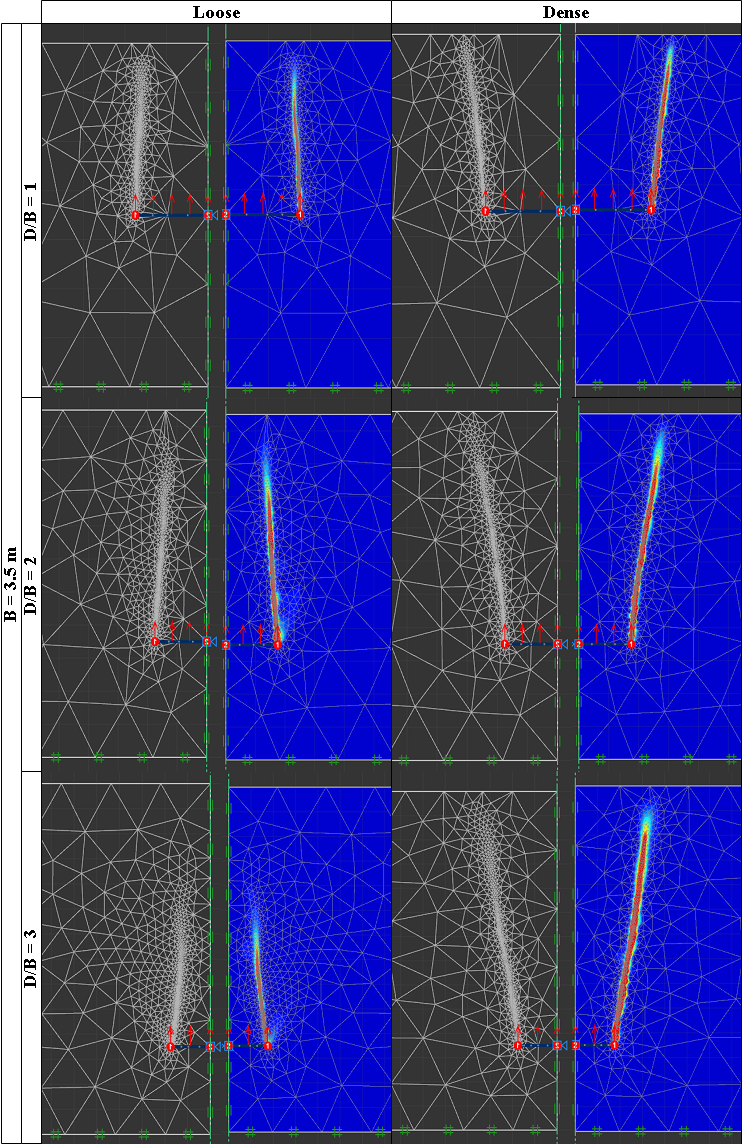
\includegraphics[width=1\linewidth]{myfigureeeeee/D_three_point_five} \caption{Shear dissipation of NA model at 10 percent of the maximum value and $B = 3.5m$}\label{fig:unnamed-chunk-28}
\end{figure}

\begin{figure}[H]
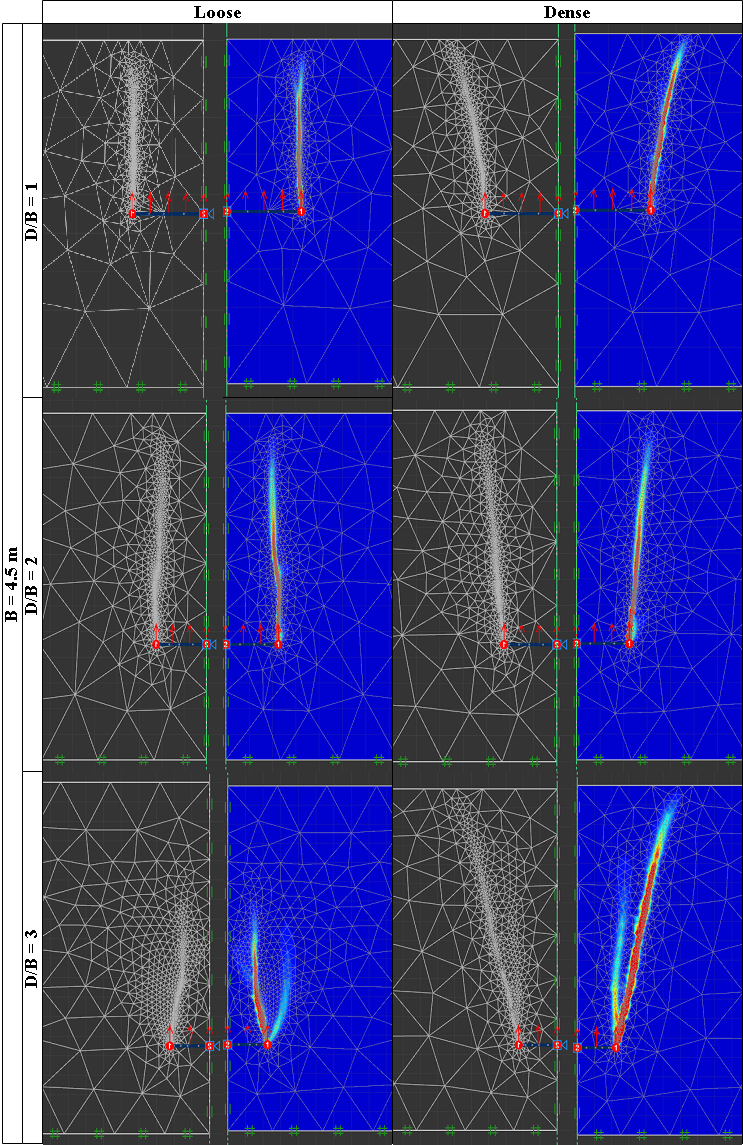
\includegraphics[width=1\linewidth]{myfigureeeeee/E_four_point_five} \caption{Shear dissipation of NA model at 10 percent of the maximum value and $B = 4.5m$}\label{fig:unnamed-chunk-29}
\end{figure}

\begin{figure}[H]
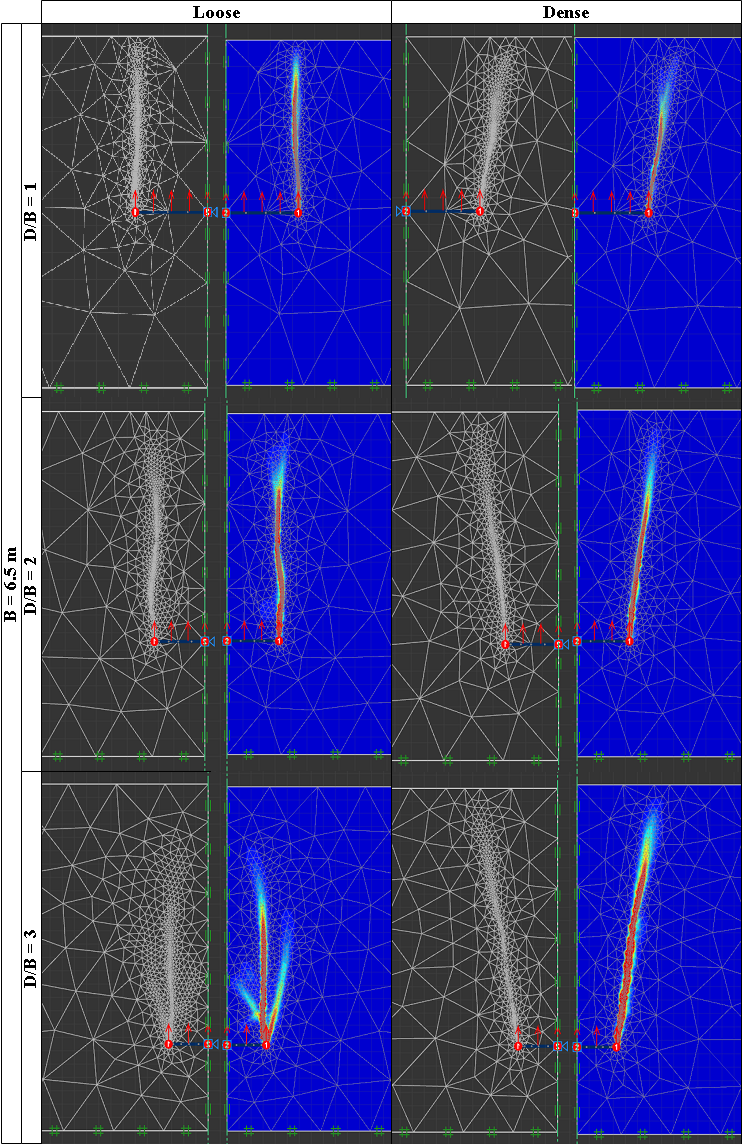
\includegraphics[width=1\linewidth]{myfigureeeeee/G_six_point_five} \caption{Shear dissipation of NA model at 10 percent of the maximum value and $B = 6.5m$}\label{fig:unnamed-chunk-30}
\end{figure}

\hypertarget{comparison-with-previous-researchers}{%
\section{Comparison with Previous Researchers}\label{comparison-with-previous-researchers}}

\begin{figure}[H]
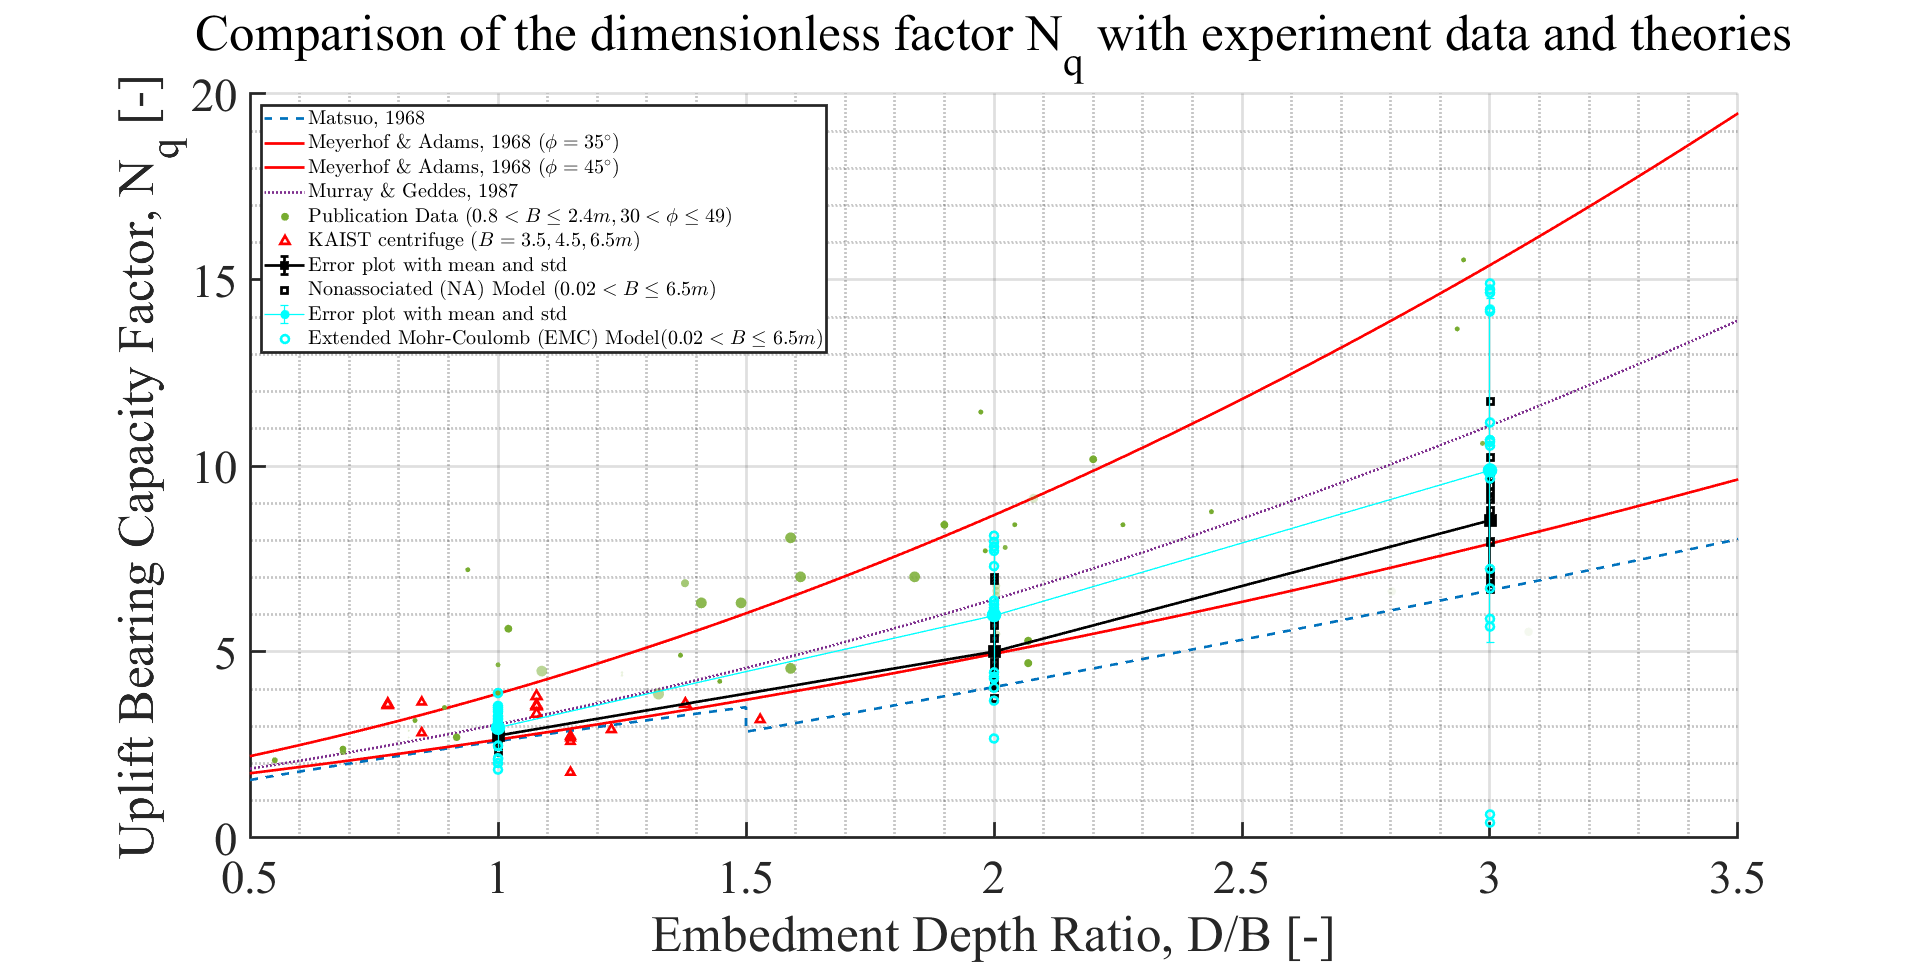
\includegraphics[width=1\linewidth]{myfigureeeeee/comparisonwiththeories} \caption{Comparison with theories and experimental data in all densities of sands}\label{fig:unnamed-chunk-31}
\end{figure}

\begin{figure}[H]
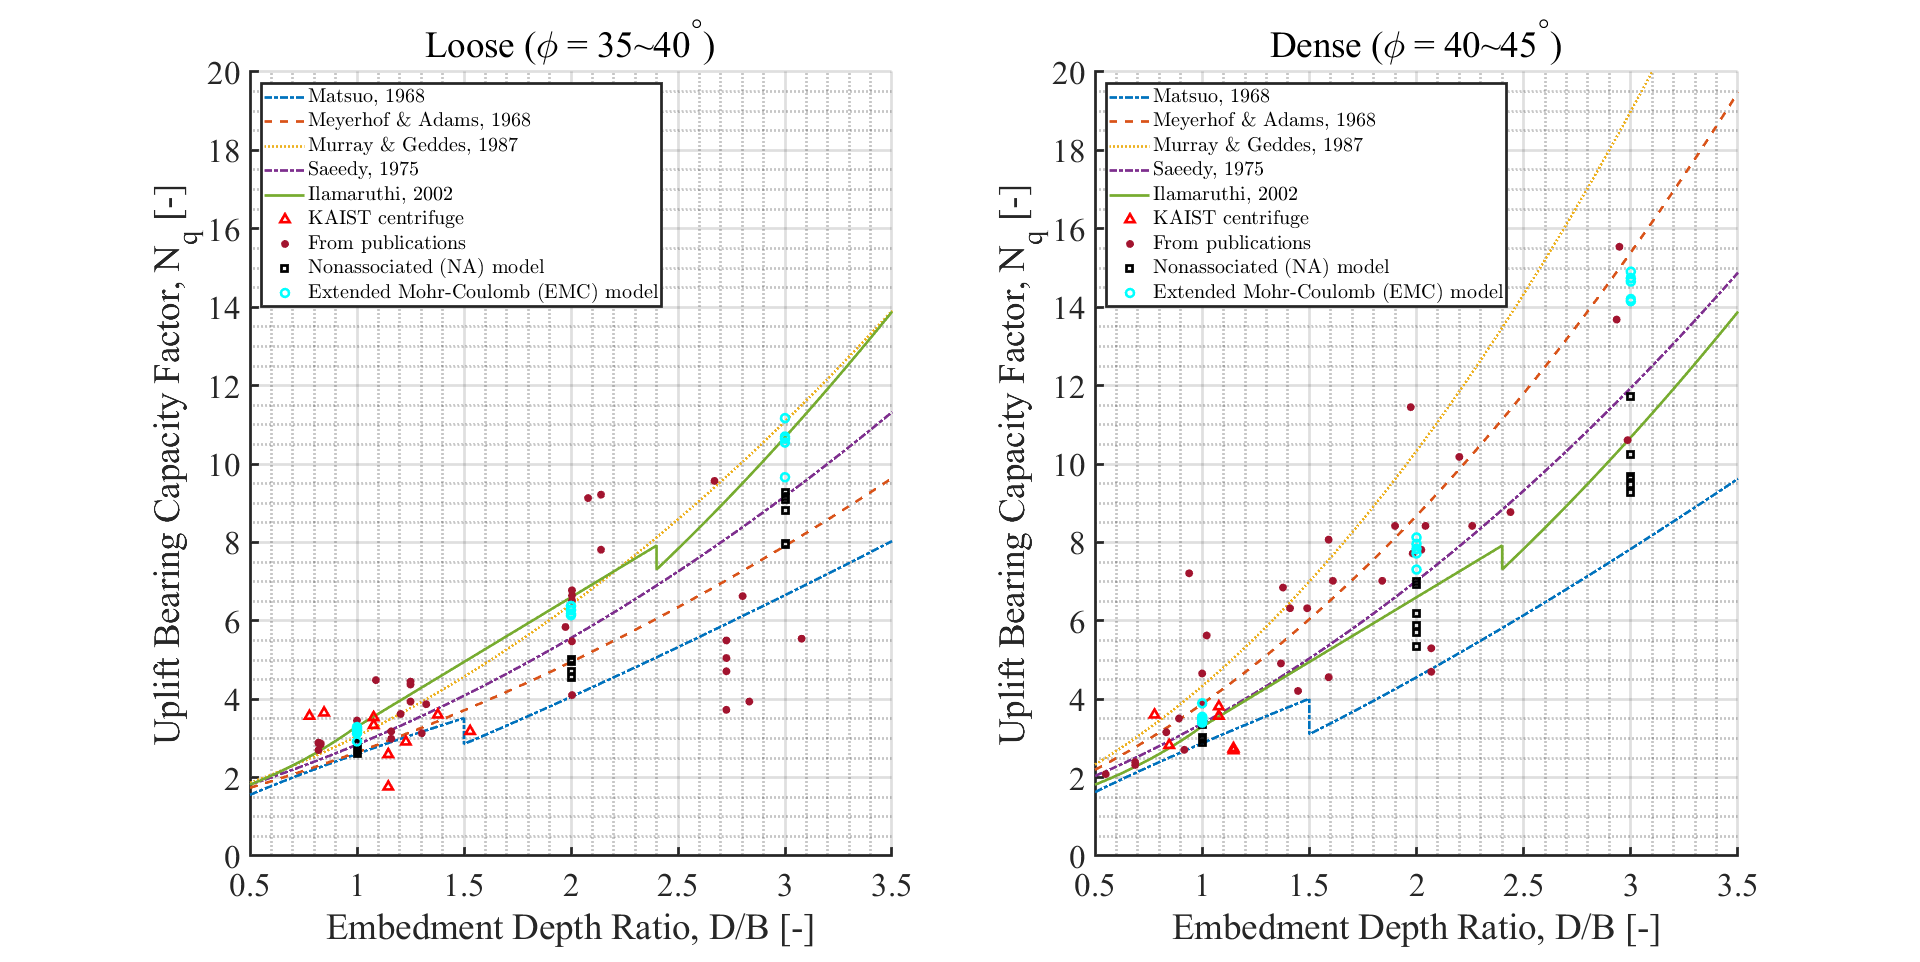
\includegraphics[width=1\linewidth]{myfigureeeeee/comparisonwiththeories_loosedense} \caption{Comparison with theories and experimental data in loose and dense sands}\label{fig:unnamed-chunk-32}
\end{figure}

\hypertarget{comparison-of-the-plot-of-the-effect-of-width-on-resistance}{%
\subsubsection{Comparison of the plot of the effect of width on resistance}\label{comparison-of-the-plot-of-the-effect-of-width-on-resistance}}

\begin{figure}[H]
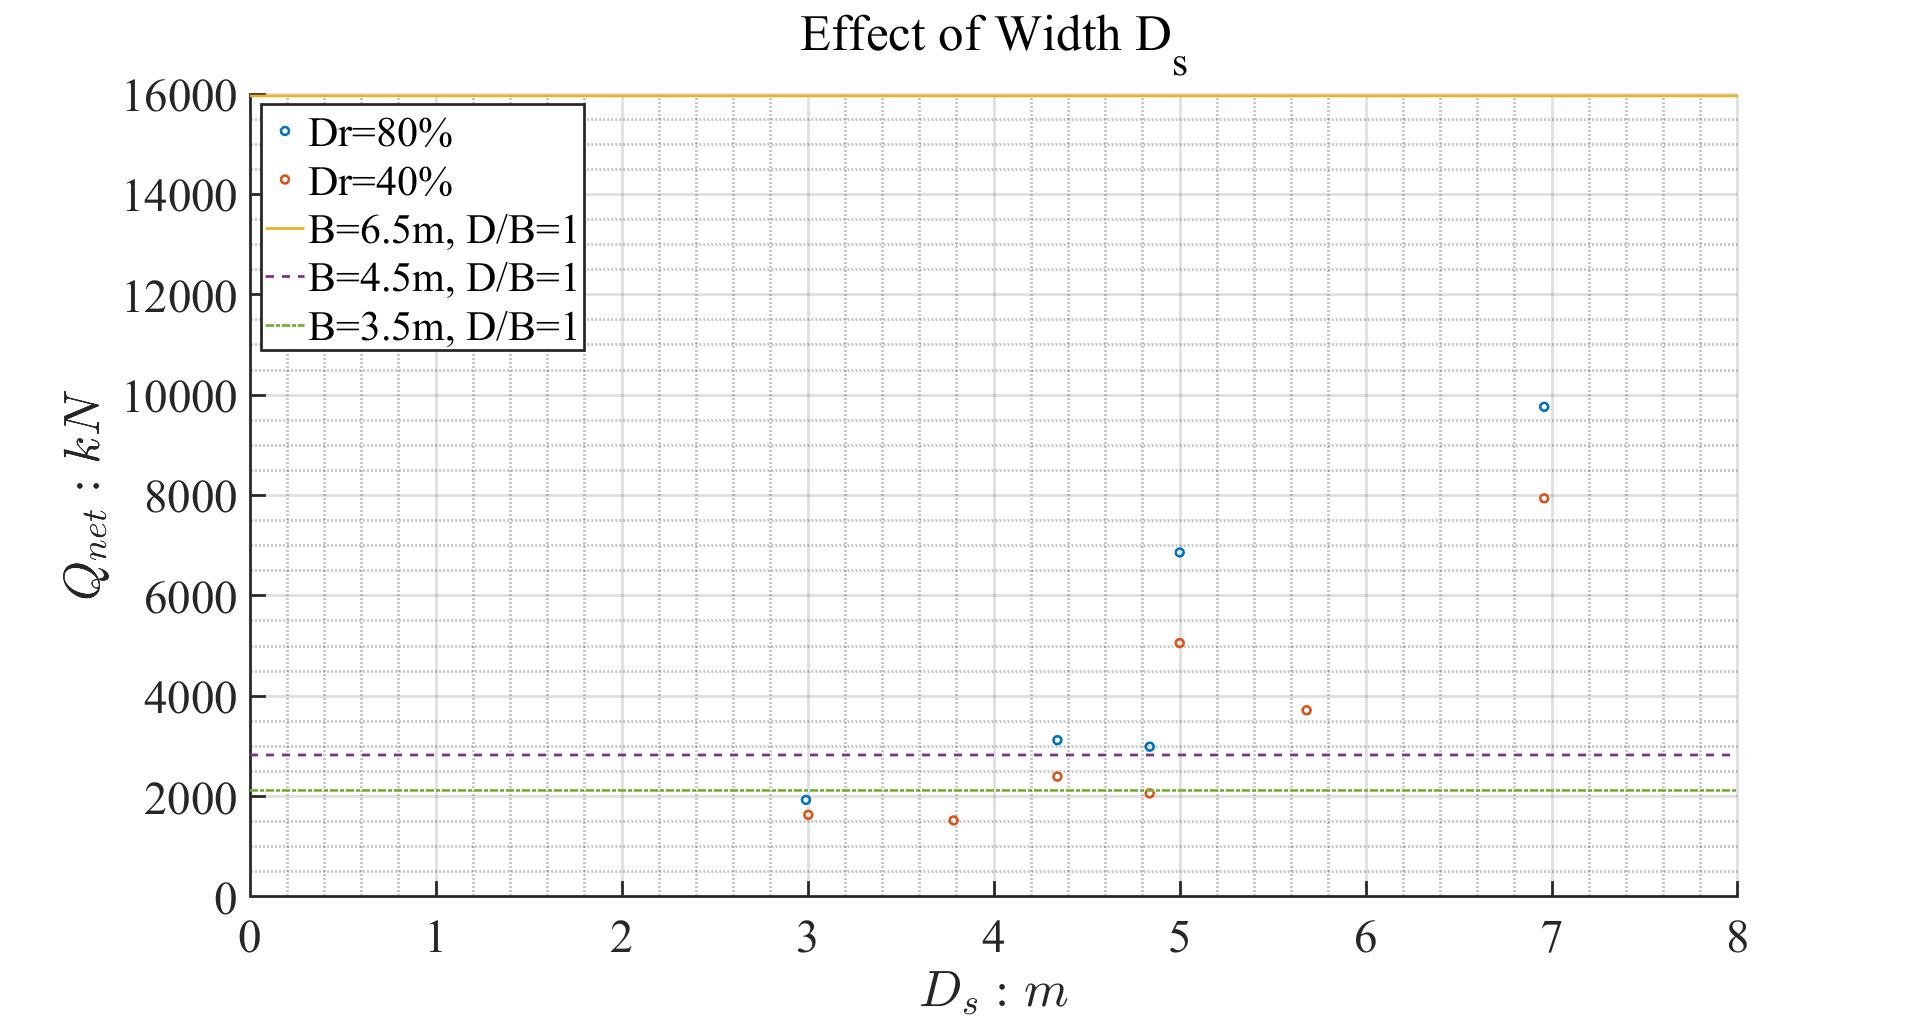
\includegraphics[width=1\linewidth]{myfigureeeeee/Comparison} \caption{Comparison drawn}\label{fig:unnamed-chunk-33}
\end{figure}

\hypertarget{comparison-with-centrifuge-experiment}{%
\chapter{Comparison with Centrifuge Experiment}\label{comparison-with-centrifuge-experiment}}

\begin{figure}[H]
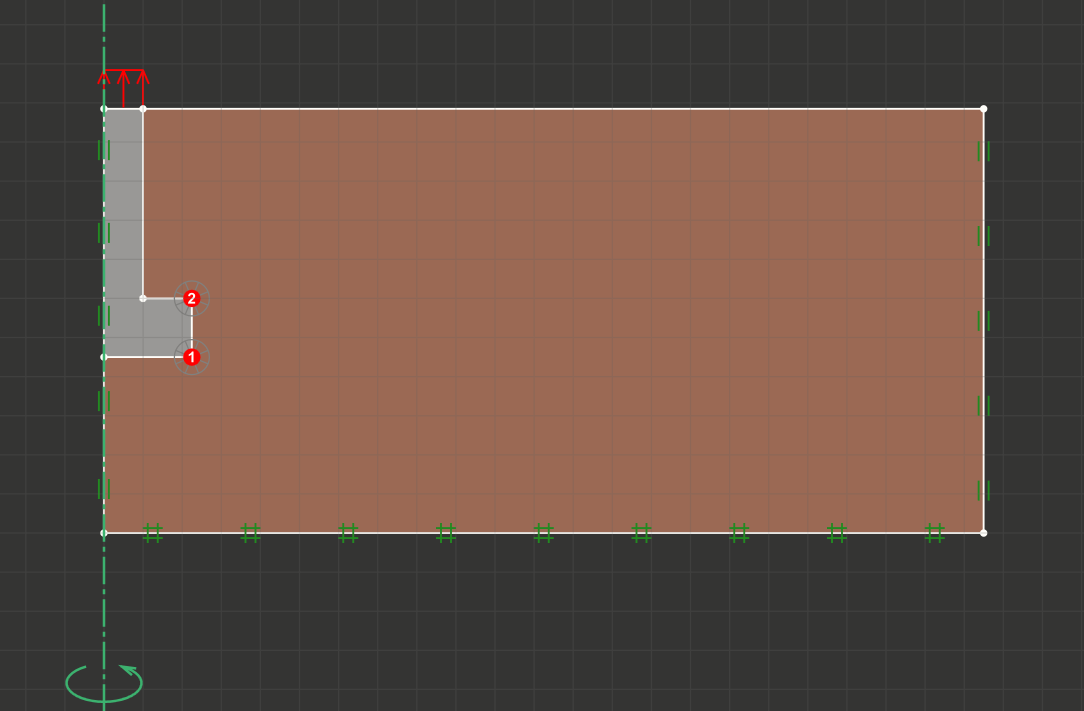
\includegraphics[width=1\linewidth]{myfigureeeeee/numericaltestsetup} \caption{Typical numerical test set-up}\label{fig:unnamed-chunk-34}
\end{figure}

\begin{longtable}[c]{@{}crrrrr@{}}
\caption{Set of varied model parameters of EMC model }
\label{tab:Set of varied model parameters of EMC model }\\
\toprule
\multicolumn{6}{c}{EMC}                                        \\* \midrule
\endfirsthead
%
\multicolumn{6}{c}%
{{\bfseries Table \thetable\ continued from previous page}} \\
\toprule
\multicolumn{6}{c}{EMC}                                        \\* \midrule
\endhead
%
\bottomrule
\endfoot
%
\endlastfoot
%
Set & \multicolumn{1}{c}{A} & \multicolumn{1}{c}{B} & \multicolumn{1}{c}{C} & \multicolumn{1}{c}{D} & \multicolumn{1}{c}{E} \\* \midrule
$E_{50} (MPa)$        & 25     & 20     & 22.5   & 35     & 40     \\
$E_{ur} (MPa)$        & 75     & 60     & 67.5   & 105    & 120    \\
$\nu_{ur}$            & 0.3    & 0.3    & 0.3    & 0.3    & 0.3    \\
$c(kPa)$              & 0      & 0      & 0      & 0      & 0      \\
$\phi(deg)$           & 37     & 34     & 35.5   & 38     & 40     \\
$\psi(deg)$           & 11     & 1      & 5      & 8      & 14     \\
$\gamma_d(kN/m3)$     & 16     & 15.5   & 15.75  & 16.5   & 17     \\
$\gamma_{sat}(kN/m3)$ & 20     & 19     & 19.5   & 20.5   & 21     \\
$K_0$                 & 0.4264 & 0.4264 & 0.4264 & 0.4264 & 0.4264 \\
$p_{ref} (kPa)$       & 100    & 100    & 100    & 100    & 100    \\
$m$                   & 0.5    & 0.5    & 0.5    & 0.5    & 0.5    \\* \bottomrule
\end{longtable}

\begin{longtable}[c]{@{}crrrrr@{}}
\caption{Set of varied model parameters for NA model}
\label{tab:my-table}\\
\toprule
\multicolumn{6}{c}{NA}                                         \\* \midrule
\endfirsthead
%
\multicolumn{6}{c}%
{{\bfseries Table \thetable\ continued from previous page}} \\
\toprule
\multicolumn{6}{c}{NA}                                         \\* \midrule
\endhead
%
\bottomrule
\endfoot
%
\endlastfoot
%
Set & \multicolumn{1}{c}{F} & \multicolumn{1}{c}{G} & \multicolumn{1}{c}{H} & \multicolumn{1}{c}{I} & \multicolumn{1}{c}{J} \\* \midrule
$E (MPa)$            & 25     & 20     & 30     & 35     & 40     \\
$\nu$                & 0.25   & 0.25   & 0.25   & 0.25   & 0.25   \\
$c (kPa)$            & 0      & 0      & 0      & 0      & 0      \\
$\phi(deg)$          & 35     & 33     & 37     & 39     & 41     \\
$\psi(deg)$          & 5      & 4      & 6      & 7      & 8      \\
$\gamma_d(kN/m3)$    & 16     & 14     & 15     & 16     & 14     \\
$\gamma_{sat}(kN/m3)$  & 20     & 19     & 19.5   & 20     & 19     \\
$K_0$                & 0.4264 & 0.4264 & 0.4264 & 0.4264 & 0.4264 \\* \bottomrule
\end{longtable}

\begin{longtable}[c]{@{}crrrr@{}}
\caption{Centrifuge test set-up and result}
\label{tab:Centrifuge test set-up and result}\\
\toprule
Case & \multicolumn{1}{c}{$B (m)$} & \multicolumn{1}{c}{$\frac{D}{B}$} & \multicolumn{1}{c}{$\gamma_{d} (kN/m^3)$} & \multicolumn{1}{c}{$Q_u (kN)$} \\* \midrule
\endfirsthead
%
\multicolumn{5}{c}%
{{\bfseries Table \thetable\ continued from previous page}} \\
\toprule
Case & \multicolumn{1}{c}{$B (m)$} & \multicolumn{1}{c}{$\frac{D}{B}$} & \multicolumn{1}{c}{$\gamma_{d} (kN/m^3)$} & \multicolumn{1}{c}{$Q_u (kN)$} \\* \midrule
\endhead
%
\bottomrule
\endfoot
%
\endlastfoot
%
1-1  & 4.5 & 1   & 13.8 & 2959  \\
1-2  & 4.5 & 1.3 & 13.8 & 3845  \\
1-3  & 4.5 & 1.3 & 13.8 & 4050  \\
2-1  & 6.5 & 1   & 14   & 7433  \\
2-2  & 6.5 & 1.3 & 14   & 10440 \\
2-3  & 6.5 & 1.3 & 14   & 10590 \\
3-1  & 4.5 & 1   & 15.3 & 3312  \\
3-2  & 4.5 & 1.3 & 15.3 & 4554  \\
3-3  & 4.5 & 1.3 & 15.3 & 4824  \\
4-1  & 6.5 & 1   & 15.3 & 9331  \\
4-2A & 6.5 & 1.3 & 15.3 & 12280 \\
4-3  & 6.5 & 1.3 & 15.3 & 12240 \\
5-1  & 3.5 & 1.3 & 14   & 1980  \\
5-2  & 3.5 & 1.6 & 14   & 2658  \\
5-3  & 4.5 & 1.6 & 14   & 5351  \\
6-3  & 3.5 & 1.6 & 15.1 & 3616  \\* \bottomrule
\end{longtable}

\begin{longtable}[c]{@{}crrrrrr@{}}
\caption{Numerical model set-up for load-displacement curve comparison}
\label{tab:Numerical model set-up for load-displacement curve comparison}\\
\toprule
Code &
  \multicolumn{1}{c}{$B (m)$} &
  \multicolumn{1}{c}{$D-t (m)$} &
  \multicolumn{1}{c}{$D (m)$} &
  \multicolumn{1}{c}{$t (m)$} &
  \multicolumn{1}{c}{$b (m)$} &
  \multicolumn{1}{c}{$A (m^2)$} \\* \midrule
\endfirsthead
%
\multicolumn{7}{c}%
{{\bfseries Table \thetable\ continued from previous page}} \\
\toprule
Code &
  \multicolumn{1}{c}{$B (m)$} &
  \multicolumn{1}{c}{$D-t (m)$} &
  \multicolumn{1}{c}{$D (m)$} &
  \multicolumn{1}{c}{$t (m)$} &
  \multicolumn{1}{c}{$b (m)$} &
  \multicolumn{1}{c}{$A (m^2)$} \\* \midrule
\endhead
%
\bottomrule
\endfoot
%
\endlastfoot
%
base2 & 6.5 & 5.95 & 7.45 & 1.5  & 1   & 39.1 \\
base3  & 6.5 & 4    & 5.5  & 1.5  & 1   & 39.1 \\
base2 & 6.5 & 5.95 & 7.45 & 1.5  & 1   & 39.1 \\
base3  & 6.5 & 4    & 5.5  & 1.5  & 1   & 39.1 \\
base2 & 6.5 & 5.95 & 7.45 & 1.5  & 1   & 39.1 \\
base2 & 6.5 & 5.95 & 7.45 & 1.5  & 1   & 39.1 \\
base2 & 6.5 & 5.95 & 7.45 & 1.5  & 1   & 39.1 \\
base6 & 4.5 & 2    & 3.5  & 1.5  & 1   & 17.1 \\
base5 & 4.5 & 3.35 & 4.85 & 1.5  & 1   & 17.1 \\
base5 & 4.5 & 3.35 & 4.85 & 1.5  & 1   & 17.1 \\
base6 & 4.5 & 2    & 3.5  & 1.5  & 1   & 17.1 \\
base5 & 4.5 & 3.35 & 4.85 & 1.5  & 1   & 17.1 \\
base5 & 4.5 & 3.35 & 4.85 & 1.5  & 1   & 17.1 \\
base4 & 4.5 & 4.7  & 6.2  & 1.5  & 1   & 17.1 \\
base8 & 3.5 & 3.55 & 4.3  & 0.75 & 0.6 & 11.1 \\
base7 & 3.5 & 4.6  & 5.35 & 0.75 & 0.6 & 11.1 \\* \bottomrule
\end{longtable}

\begin{figure}[H]
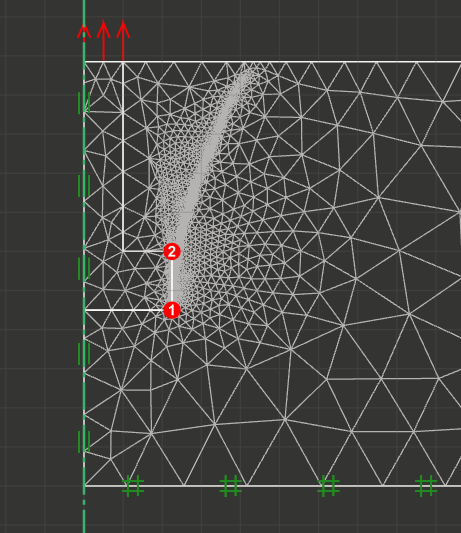
\includegraphics[width=1\linewidth]{myfigureeeeee/typicalresult2} \caption{Typical mesh of the numerical simulation; number of mesh = 5000}\label{fig:unnamed-chunk-35}
\end{figure}

\begin{figure}[H]
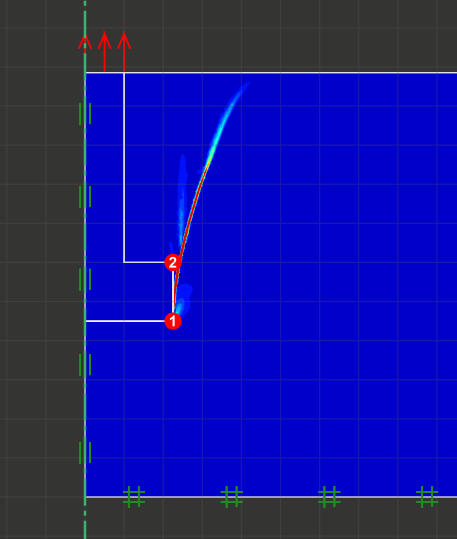
\includegraphics[width=1\linewidth]{myfigureeeeee/typicalresult} \caption{Typical result of the numerical simulation; 1st decile of the shear dissipation (kJ)}\label{fig:unnamed-chunk-36}
\end{figure}

\hypertarget{results-of-numerical-analysis-for-finding-the-model-that-fits-the-centrifuge-loaddisplacement-curve}{%
\subsubsection{Results of numerical analysis for finding the model that fits the centrifuge load---displacement curve}\label{results-of-numerical-analysis-for-finding-the-model-that-fits-the-centrifuge-loaddisplacement-curve}}

\begin{figure}[H]
\includegraphics[width=1\linewidth]{myfigureeeeee/BASE2} \caption{Code name base2; B=6.5m; B/D = 0.915}\label{fig:unnamed-chunk-37}
\end{figure}

\begin{figure}[H]
\includegraphics[width=1\linewidth]{myfigureeeeee/BASE3} \caption{Code name base3; B=6.5m; B/D = 0.615}\label{fig:unnamed-chunk-38}
\end{figure}

\begin{figure}[H]
\includegraphics[width=1\linewidth]{myfigureeeeee/BASE4} \caption{Code name base4; B=4.5m; B/D = 1.044}\label{fig:unnamed-chunk-39}
\end{figure}

\begin{figure}[H]
\includegraphics[width=1\linewidth]{myfigureeeeee/BASE5} \caption{Code name base5; B=4.5m; B/D = 0.744}\label{fig:unnamed-chunk-40}
\end{figure}

\begin{figure}[H]
\includegraphics[width=1\linewidth]{myfigureeeeee/BASE6} \caption{Code name base6; B=4.5m; B/D = 0.444}\label{fig:unnamed-chunk-41}
\end{figure}

\begin{figure}[H]
\includegraphics[width=1\linewidth]{myfigureeeeee/BASE7} \caption{Code name base7; B=3.5m; B/D = 1.314}\label{fig:unnamed-chunk-42}
\end{figure}

\begin{figure}[H]
\includegraphics[width=1\linewidth]{myfigureeeeee/BASE8} \caption{Code name base8; B=3.5m; B/D = 0.101}\label{fig:unnamed-chunk-43}
\end{figure}

\hypertarget{determination-of-model-parameters}{%
\subsubsection{Determination of model parameters}\label{determination-of-model-parameters}}

To evaluate the difference between the centrifuge test result and the model prediction, residual error was used:

\[
Error = \lvert \frac{y_{actual}-y_{estimated}}{y_{actual}}\lvert \times 100\% 
\]
The goal is to find the model which best fits (or has the least error) the measured data.
For the dense sand cases, Model C and H, whereas for the loose sand cases, Model B and G were chosen for the further studies.

\begin{figure}[H]
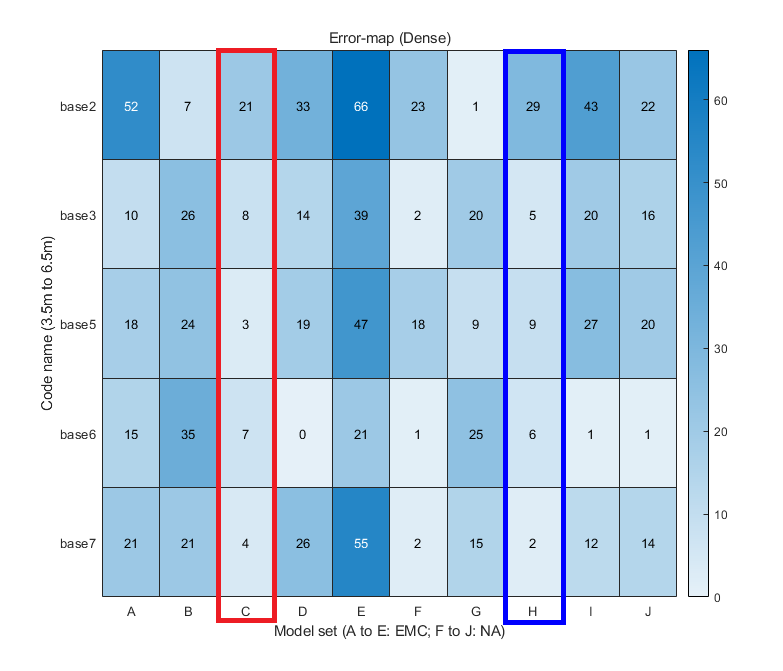
\includegraphics[width=1\linewidth]{myfigureeeeee/errormap_emc} \caption{Heat-map of errors between cetrifuge test and model (dense cases); model C and H were selected among available 10 models}\label{fig:unnamed-chunk-44}
\end{figure}

\begin{figure}[H]
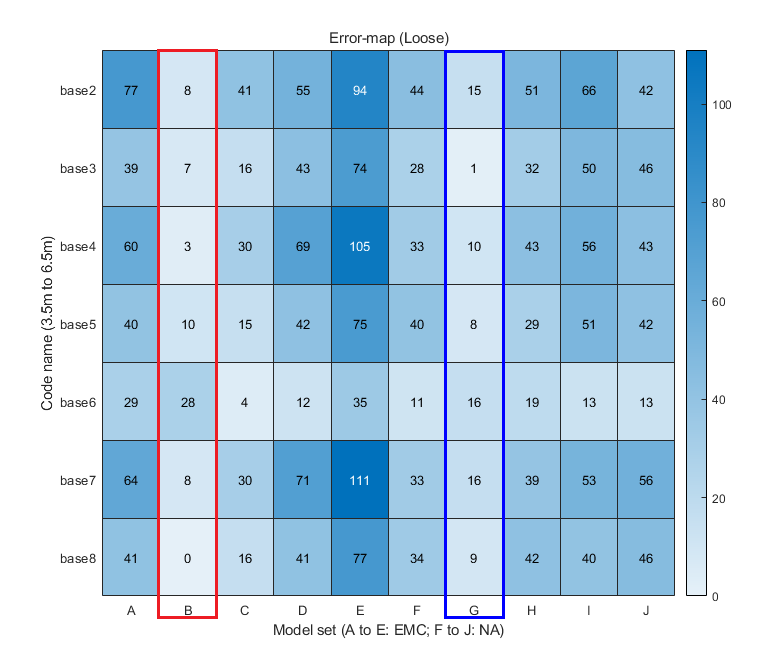
\includegraphics[width=1\linewidth]{myfigureeeeee/errormap_emc2} \caption{Heat-map of errors between cetrifuge test and model (loose cases); model B and G were selected among 10 available models}\label{fig:unnamed-chunk-45}
\end{figure}

\hypertarget{comparison-of-the-centrifuge-test-results-with-the-chosen-model}{%
\section{Comparison of the centrifuge test results with the chosen model}\label{comparison-of-the-centrifuge-test-results-with-the-chosen-model}}

\begin{figure}[H]
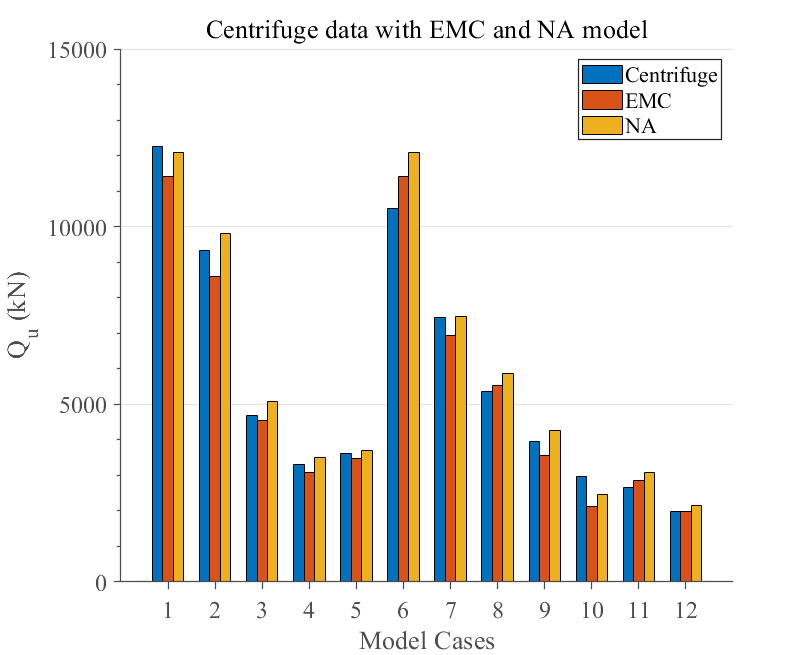
\includegraphics[width=1\linewidth]{myfigureeeeee/barchart1} \caption{Bar-chart of centrifuge test and model (all cases); from left to right, 1: B=6.5m,D/B=1.3; 2: B=6.5m,D/B=1; 3: B=4.5m,D/B=1.3; 4: B=4.5m,D/B=1; 5: B=3.5m,D/B=1.6; 6: B=6.5m,D/B=1.3; 7: B=6.5m,D/B=1; 8: B=4.5m,D/B=1.6; 9: B=4.5m,D/B=1.3; 10: B=4.5m,D/B=1; 11: B=3.5m,D/B=1.6; 12: B=3.5m,D/B=1.3}\label{fig:unnamed-chunk-46}
\end{figure}

\begin{landscape}

\hypertarget{result-of-loaddisplacement-curves-of-the-centrifuge-measurement-with-emc-and-na-models}{%
\subsubsection{Result of load---displacement curves of the centrifuge measurement with EMC and NA models}\label{result-of-loaddisplacement-curves-of-the-centrifuge-measurement-with-emc-and-na-models}}

\begin{figure}[H]
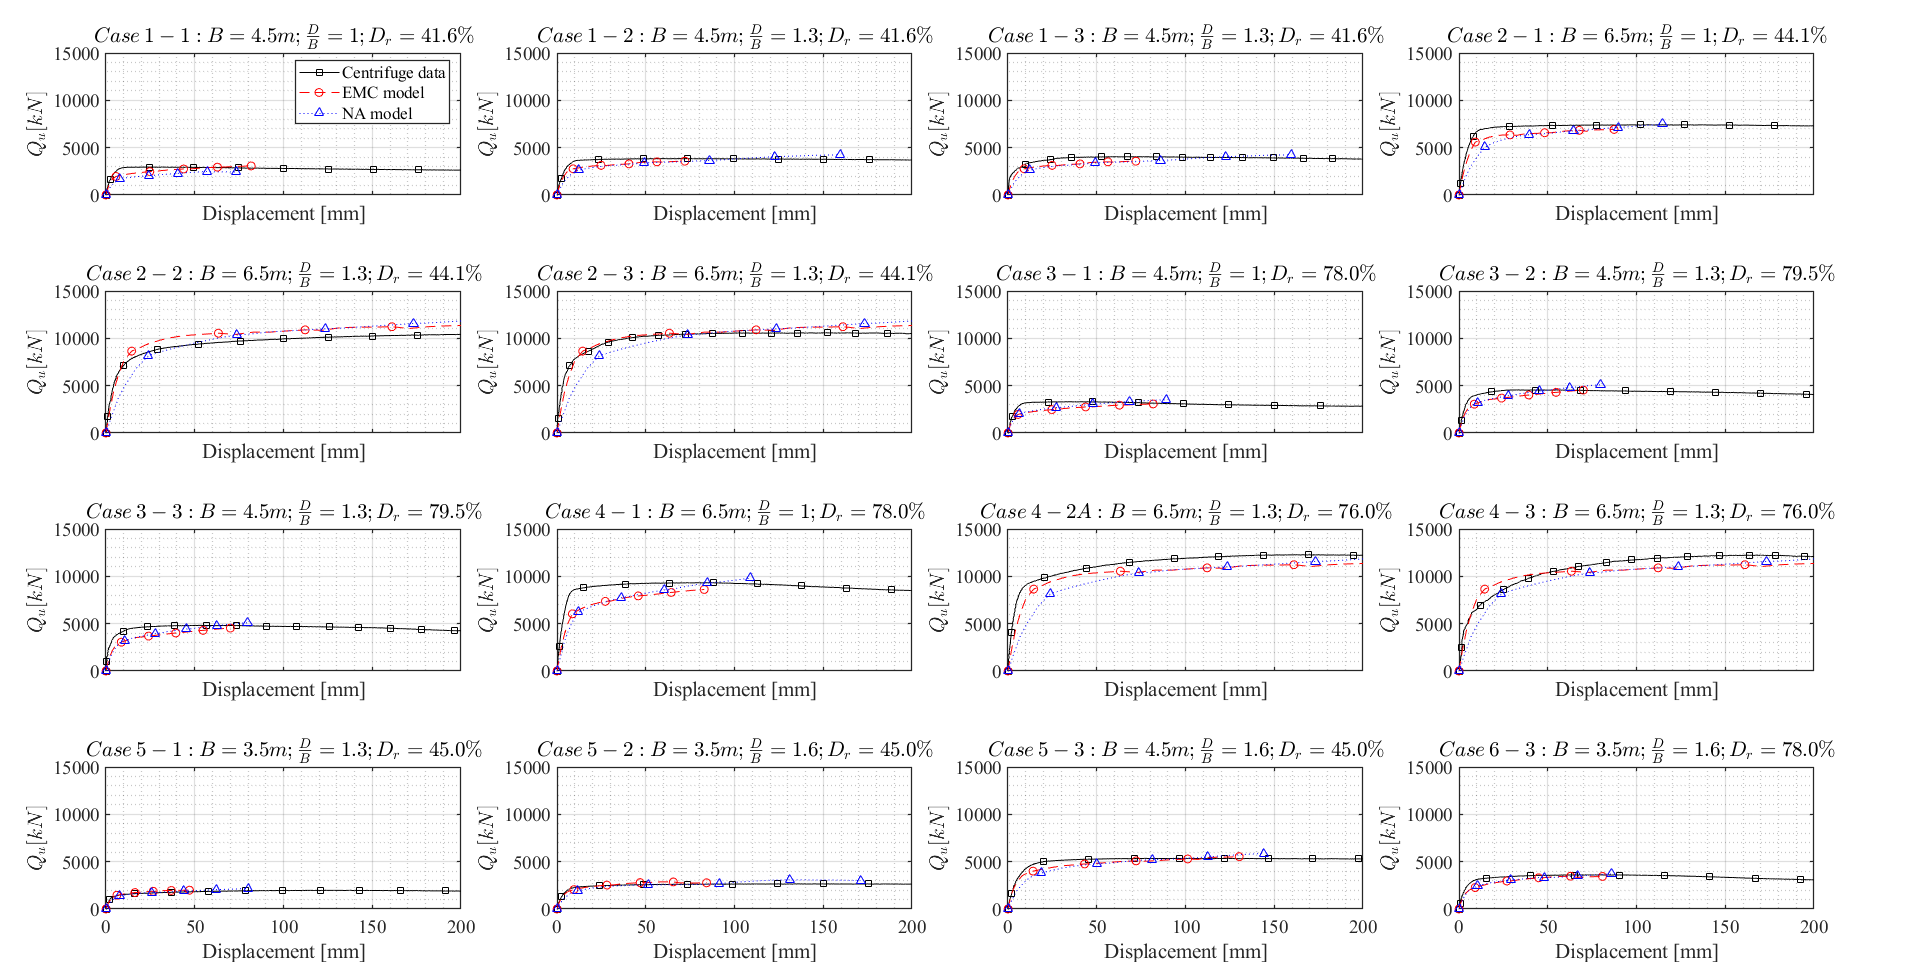
\includegraphics[width=1\linewidth]{myfigureeeeee/Comparison_of_centrifuge_data_with_EMC_and_NA_models} \caption{Comparison of centrifuge data with EMC and NA models}\label{fig:unnamed-chunk-47}
\end{figure}

\end{landscape}

\startappendices

\begin{landscape}

\hypertarget{list-of-loaddisplacement-curves}{%
\chapter{List of Load---Displacement Curves}\label{list-of-loaddisplacement-curves}}

\begin{figure}[H]
\includegraphics[width=1\linewidth]{myfigureeeeee/CodeA} \caption{Cumulative load-displacement curves of uplift of plate anchor in loose, medium, dense sands; D/B = 1,2,3; B=0.02m }\label{fig:unnamed-chunk-48}
\end{figure}

\begin{figure}[H]
\includegraphics[width=1\linewidth]{myfigureeeeee/CodeB} \caption{Cumulative load-displacement curves of uplift of plate anchor in loose, medium, dense sands; D/B = 1,2,3; B=0.2m}\label{fig:unnamed-chunk-49}
\end{figure}

\begin{figure}[H]
\includegraphics[width=1\linewidth]{myfigureeeeee/CodeC} \caption{Cumulative load-displacement curves of uplift of plate anchor in loose, medium, dense sands; D/B = 1,2,3; B=1.0m}\label{fig:unnamed-chunk-50}
\end{figure}

\begin{figure}[H]
\includegraphics[width=1\linewidth]{myfigureeeeee/CodeD} \caption{Cumulative load-displacement curves of uplift of plate anchor in loose, medium, dense sands; D/B = 1,2,3; B=3.5m}\label{fig:unnamed-chunk-51}
\end{figure}

\begin{figure}[H]
\includegraphics[width=1\linewidth]{myfigureeeeee/CodeE} \caption{Cumulative load-displacement curves of uplift of plate anchor in loose, medium, dense sands; D/B = 1,2,3; B=4.5m}\label{fig:unnamed-chunk-52}
\end{figure}

\begin{figure}[H]
\includegraphics[width=1\linewidth]{myfigureeeeee/CodeG} \caption{Cumulative load-displacement curves of uplift of plate anchor in loose, medium, dense sands; D/B = 1,2,3; B=6.5m}\label{fig:unnamed-chunk-53}
\end{figure}

\end{landscape}

\hypertarget{references}{%
\chapter{REFERENCES}\label{references}}

Wood, D. M. (2017). Geotechnical modelling. CRC press.

Doherty, J. P., \& Muir Wood, D. (2013). An extended Mohr--Coulomb (EMC) model for predicting the settlement of shallow foundations on sand. Géotechnique, 63(8), 661-673.

Gajo, A., \& Wood, M. (1999). Severn--Trent sand: a kinematic-hardening constitutive model: the q--p formulation. Géotechnique, 49(5), 595-614.

Krabbenhoft, S., Krabbenhoft, K., \& Christensen, R. Limit analysis of the bearing capacity of strip-and circular footings on a layer of sand overlying clay.

Sakai, T., \& Tanaka, T. (2007). Experimental and numerical study of uplift behavior of shallow circular anchor in two-layered sand. Journal of geotechnical and geoenvironmental engineering, 133(4), 469-477.

Tanaka, T., \& Sakai, T. (1993). Progressive failure and scale effect of trap-door problems with granular materials. Soils and Foundations, 33(1), 11-22.

Sakai, T., \& Tanaka, T. (1998). Scale effect of a shallow circular anchor in dense sand. Soils and Foundations, 38(2), 93-99.

Sakai, T., \& Tanaka, T. (2007). Experimental and numerical study of uplift behavior of shallow circular anchor in two-layered sand. Journal of geotechnical and geoenvironmental engineering, 133(4), 469-477.

Riyad, A. S. M., Rokonuzzaman, M., \& Sakai, T. (2020). Progressive failure and scale effect of anchor foundations in sand. Ocean Engineering, 195, 106496.

Kumar, J., \& Kouzer, K. M. (2008). Vertical uplift capacity of horizontal anchors using upper bound limit analysis and finite elements. Canadian Geotechnical Journal, 45(5), 698-704.

Riyad, A. S. M., Rokonuzzaman, M., \& Sakai, T. (2020). Effect of using different approximation models to the exact Mohr--Coulomb material model in the FE simulation of Anchor Foundations in sand. International Journal of Geo-Engineering, 11(1), 1-21.

Riyad, A. S. M., Rokonuzzaman, M., \& Sakai, T. (2020). Progressive failure and scale effect of anchor foundations in sand. Ocean Engineering, 195, 106496.

Roy, A., Chow, S. H., O'Loughlin, C. D., \& Randolph, M. F. (2021). Towards a simple and reliable method for calculating uplift capacity of plate anchors in sand. Canadian Geotechnical Journal, 58(9), 1314-1333.


%%%%% REFERENCES
\setlength{\baselineskip}{0pt} % JEM: Single-space References

{\renewcommand*\MakeUppercase[1]{#1}%
\printbibliography[heading=bibintoc,title={\bibtitle}]}


\end{document}
